\documentclass{article}

\usepackage{amsmath}
\usepackage{natbib}
\usepackage{graphicx}
\usepackage{siunitx}
\usepackage{float}
\newcommand\tab[1][1cm]{\hspace*{#1}}
\date{} 
\addtolength{\jot}{3}
\begin{document}





\begin{figure}[H]
\vspace{-10mm}

\includegraphics[scale=0.8]{ee.png}


\vfil
\hfil \Large \bf MIDDLE EAST TECHNICAL UNIVERSITY
 \hfil
\vfil

\vspace{5mm}
\vfil
\hfil \large \bf  EE464- STATIC POWER CONVERSION-II
 \hfil
\vfil

\vspace{5mm}
\vfil
\hfil \large \bf Hardware Project Final Report\hfil
\vfil
\bf

\vspace{23mm}

Deniz Boran KARACA    2093987
\newline

Mert Yaşar AYDIN \tab2093334
\newline

Canberk DUMAN \tab 2030450


\vspace{5mm}
\small Date: 24/06/2020


\end{figure}
\newpage

\renewcommand*\contentsname{Table of Content}
\tableofcontents
\newpage
\section{Introduction}

This report is prepared to provide design specifications, component selections, performance and computer simulations of the our isolated flyback converter design for the EE464 hardware project. All deliverables  of the project which are isolated flyback converter, compensator, controller and thermal designs will be provided in this report.
\newline
There are mainly two different topologies and three different specs for each topology. As XXX we have chosen the Flyback #1 topology whose specs are listed below:
\begin{figure}[H]
    \centering
    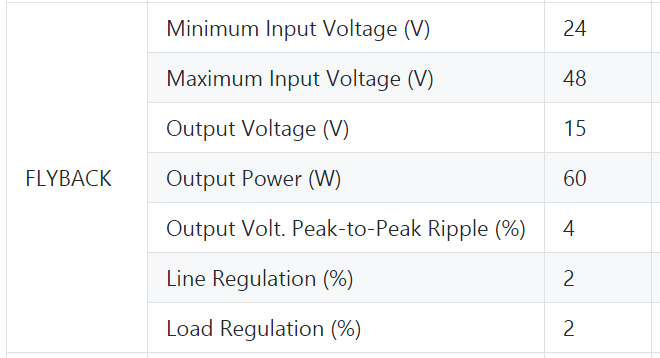
\includegraphics[scale=0.5]{f5.png}
    \caption{Design Specifications of the Flyback 1 Converter}
    \label{fig:my_label}
\end{figure}

 Simplicity of less components, wide input voltage range and lower cost advantages of Flyback topology are the main reasons of our choice. Compact design and high power density is another benefits of the Flyback converter. Moreover, the Flyback converter offers higher efficiency in low voltage range. The Flyback #1 topology is preferred by taking all of these into account.
 
 
\section{Isolated Flyback Converter Design and Component Selections}
A Flyback converter has two kinds of operation modes ; continuous conduction mode (CCM) and discontinuous conduction mode (DCM). CCM and DCM have their own advantages and disadvantages, respectively.\\
A CCM flyback was preferred for this project for improved efficiency, reduced
component stress and reduced filter size. A CCM flyback operation reduces peak currents, RMS
currents, and switch loss. Therefore CCM is usually recommended for low voltage
and high current output applications. However the main disadvantage of a CCM flyback is the lower control loop bandwidth due to a right-half plane zero (RHPZ) which can be solved by a compensator. 

\begin{figure}[H]
    \centering
    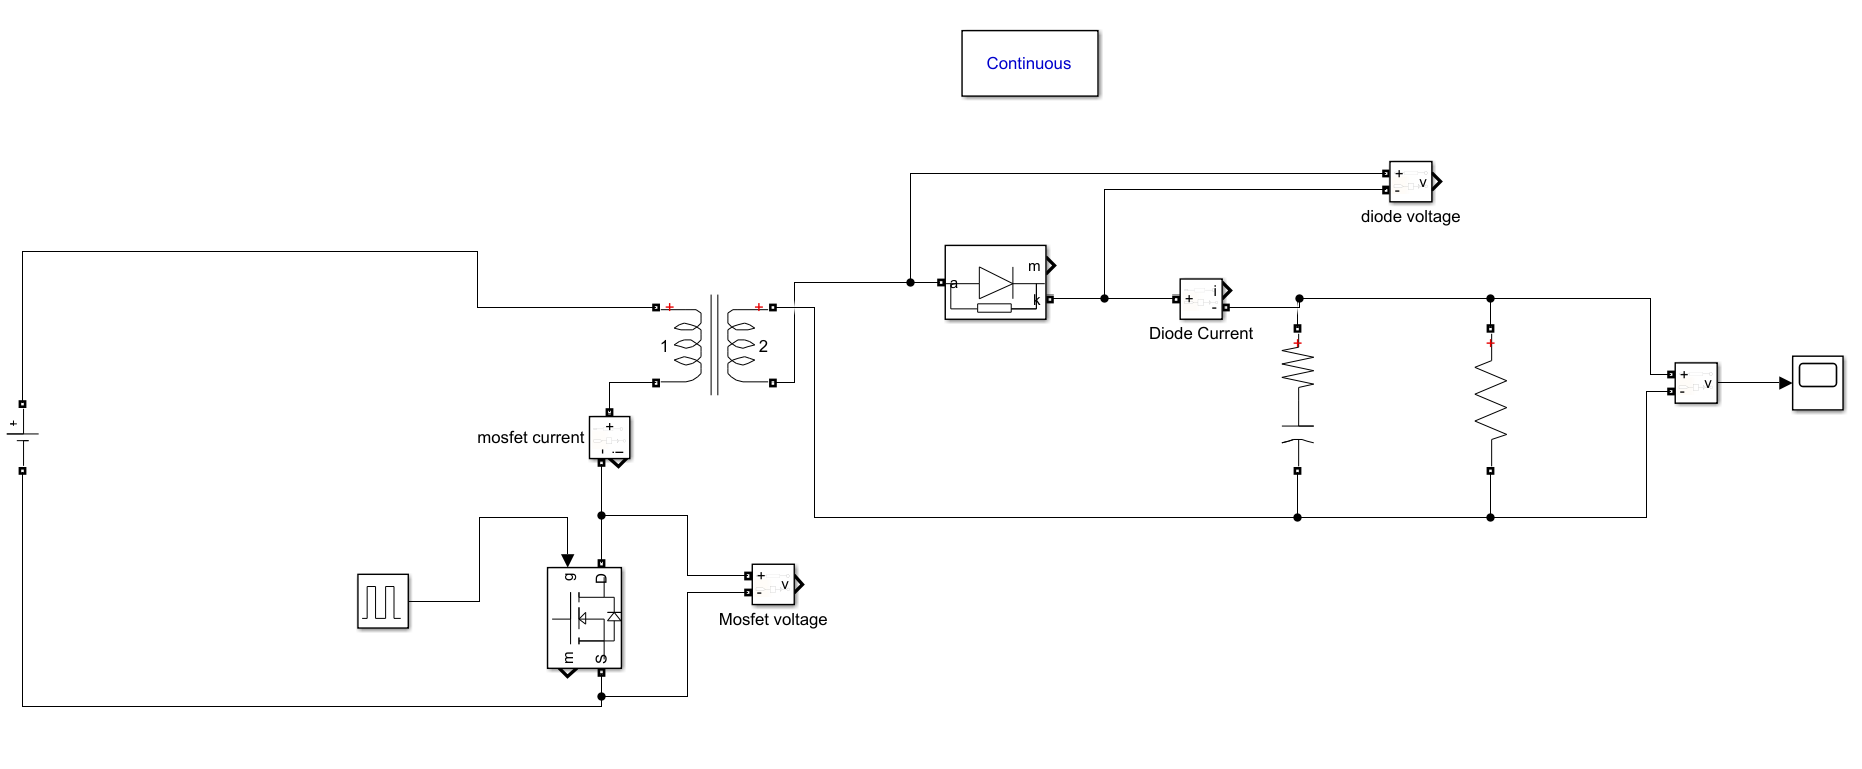
\includegraphics[scale=0.3]{f10.png}
    \caption{The framework design of Flyback converter.}
    \label{fig:my_label}
\end{figure}

Let's start by choosing turn ratio of transformer and estimated efficiency: 
\begin{gather*}
    N=\frac{N_{primary}}{N_{secondary}}=1.5\\
    \eta = \frac{P_{out}}{P_{in}}\approx \%80\\
    Hence, \tab P_{in}= 75W\\
\end{gather*}
\
\begin{gather*}
    D_{max} = 0.5 \\
    V_D=0.5 \: \text{diode forward voltage}\\
    N=\frac{N_1}{N_2}=\frac{V_{in, min}D_{max}}{(V_{out}+V_D)(1-D_{max})}=1.548\\
    \frac{1-D_{min}}{D_{min}}=\frac{V_{max}}{(V_{out}+V_D)n}\\
    D_{min}=0.326
\end{gather*}

\newline

\subsection{Framework Design}
Switched mode power supply (SMPS) design is
inherently a very complex job requires many trade-off decisions
and iterations with a lot of design parameters. In design process, we have comprehensively worked on literature and step-by-step notes. The framework of our design is build by following 3 steps: 




\begin{enumerate}
  \item Determine $V_{Mosfet}$:
  \begin{gather*}
      V_{Mosfet}=V_{in, max}+n(V_{out}+V_D)\approx 72V\\
      where \: V_D=diode(schottky)\, voltage=0.5V\\
  \end{gather*}

  \item Determine the transformer primary side inductance $L_m$:
  
  \begin{gather*}
      L_m=\frac{(V_{DC, min}D_{max})^2}{2P_{in}f_sK} \\ 
      where \: K =0.3\text{the ripple factor in full load and minimum input voltage condition}\\
      f_s = 40kHz\\
      L_m=\frac{(24*0.5)^2}{2*75*4*10^4*0.3}\approx 78\mu H
  \end{gather*}
  Check CCM to DCM boundary: 
  \begin{gather*}
      (L_m)_{min}=\frac{(1-D)^2R}{2f}N^2=47.9\mu H\\
      L_m>(L_m)_{min}\\
  \end{gather*}
  
  \item  Determine the switch current rating:
  
  \begin{gather*}
      I_{ds, peak}= I_{EDC}+\frac{\Delta I}{2} \\
      I_{EDC}=\frac{P_{in}}{V_{in, min}D_{max}}=\frac{75}{24*0.5}=6.25A\\
      \Delta I=\frac{V_{in, min}D_{max}}{L_mf_s}=3.84A\\
      I_{ds, peak}= 8.2A\\
      I_{ds, rms}=\sqrt{[3(I_{EDC})^2+(\frac{\Delta I}{2})^2]\frac{D_{max}}{3}}=4.49A\\
      I_{Mosfet}=8.5A\\
  \end{gather*}
  
 
\end{enumerate}
    
\subsection{Transformer Design}


\begin{figure}[H]
     \centering
     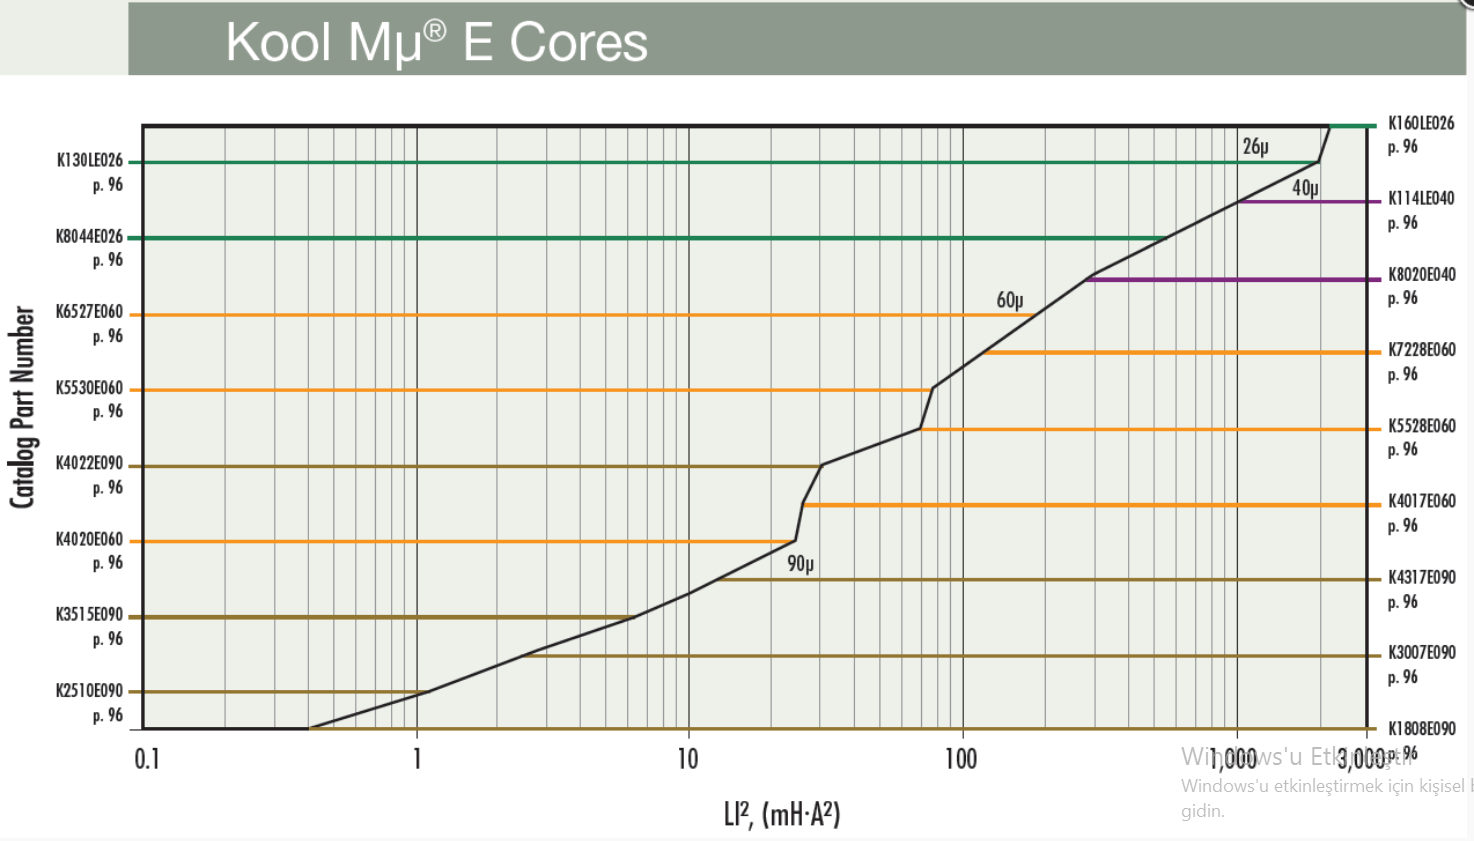
\includegraphics[scale=0.35]{f6.png}
     \caption{$LI^2$ Characteristics of Kool Mu E Cores [1]}
     \label{fig:my_label}
 \end{figure}
 
 \begin{gather*}
     L_mI^2=78*10^{-3}(2.66)^2=0.554mHA^2\\
     \text{From Figure 3 K2510E090 has been chosen}\\
     N_{pri}=\sqrt{\frac{L_{pri}}{A_L}}=\sqrt{\frac{78\mu H}{92nH/T^2}}=29turns\\
     \text{Let's choose $N_{pri}=30$}\\
     \text{Checking DC bias:}\\
     NI_{pri}=30*2.66=79.8A*turns\\
     \text{For 78.8 A*turns, $A_L=85 nH/T^2$}\\
     L=N^2A_L=30^2*85=76.5\mu H\\
     H=\frac{NI}{L_e}=\frac{30*2.66}{4.85}=16.45 A*turns/cm\\
     B=0.12 Tesla\\
 \end{gather*}
 
 \begin{figure}[H]
     \centering
     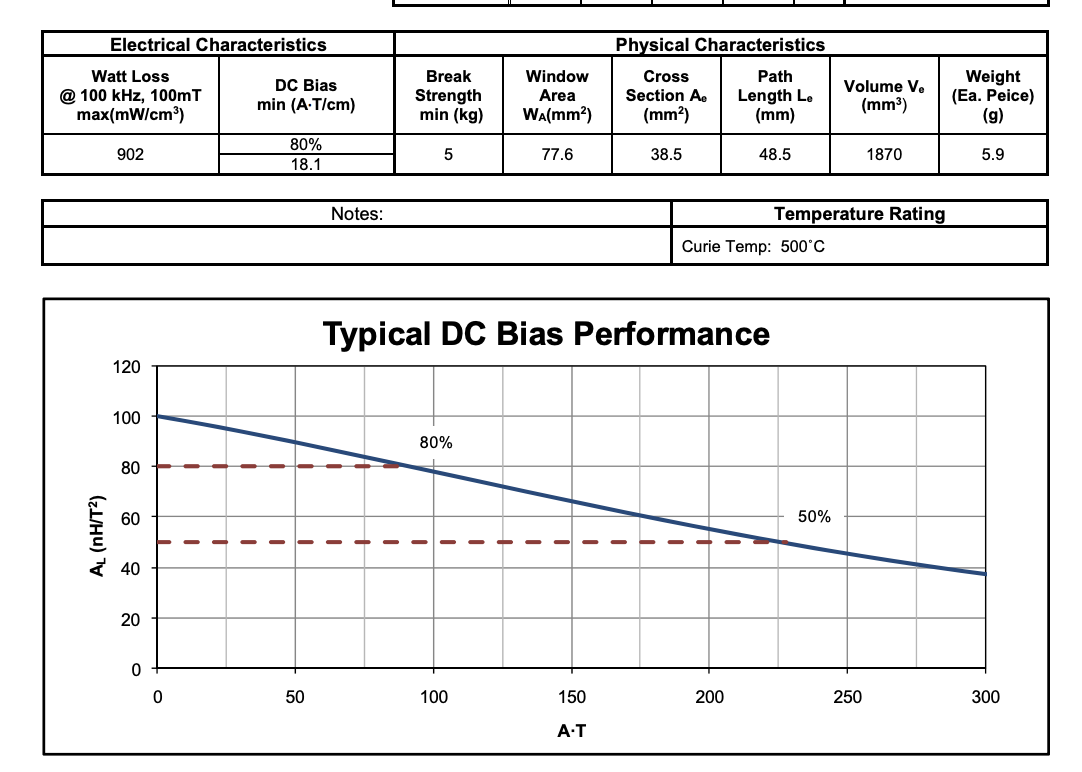
\includegraphics[scale=0.6]{CORE.png}
     \caption{Electrical characteristic of K2510E090 core.}
     \label{fig:my_label}
 \end{figure}
 
 
 \begin{figure}[H]
     \centering
     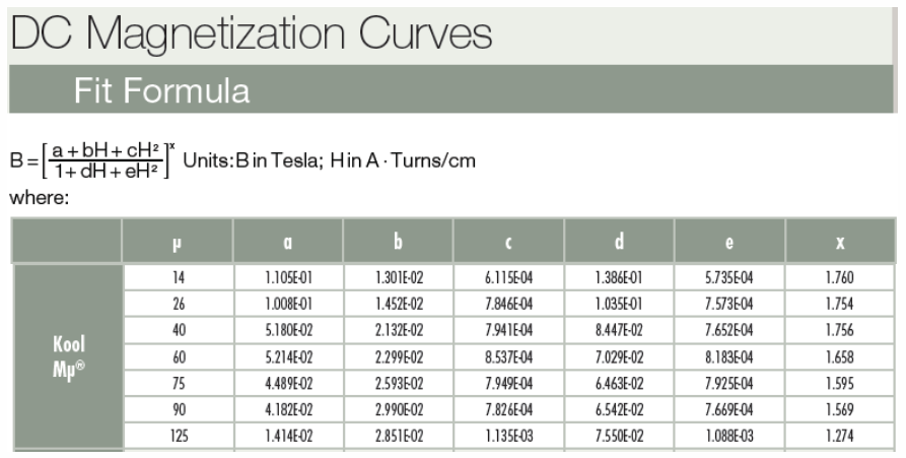
\includegraphics[scale=0.7]{z1.png}
     \caption{DC magnetization curve provided by producer.}
     \label{fig:my_label}
 \end{figure}
 
 
 $B=0.176T$ according to provided equation in Figure 5. 
 
 
 
 
  \begin{figure}[H]
     \centering
     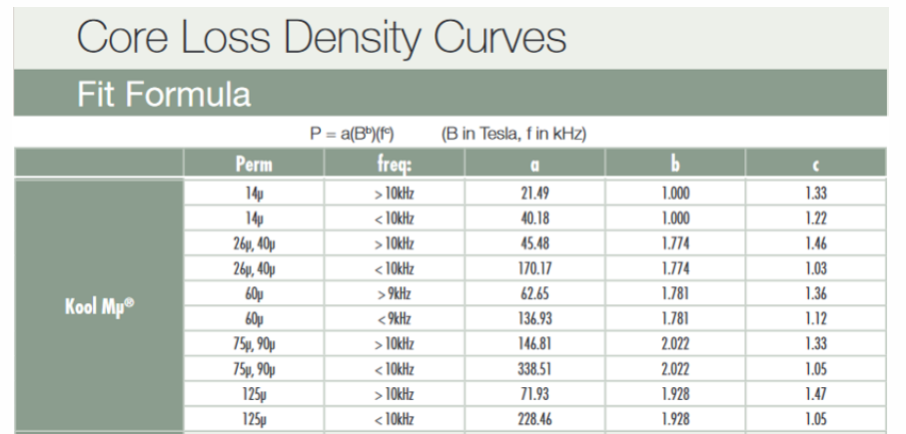
\includegraphics[scale=0.7]{z2.png}
     \caption{Core loss density curve provided by producer.}
     \label{fig:my_label}
 \end{figure}
 \begin{gather*}
      P=568.8 mW/cm^3\\
    \text{Volume of selected core=}1.87 cm^3\\
    \text{Therefore core loss=}568.8*1.87=1.063W\\
 \end{gather*}

 
 
 
 
 \newpage
 
 
 \subsection{Wire Selection}
 Skin effect and switching frequency are considered for wire selection. Therefore, possible maximum conductor cross section was chosen to avoid high ac resistance and losses, as seen in Figure 7.
 
 \begin{figure}[H]
     \centering
     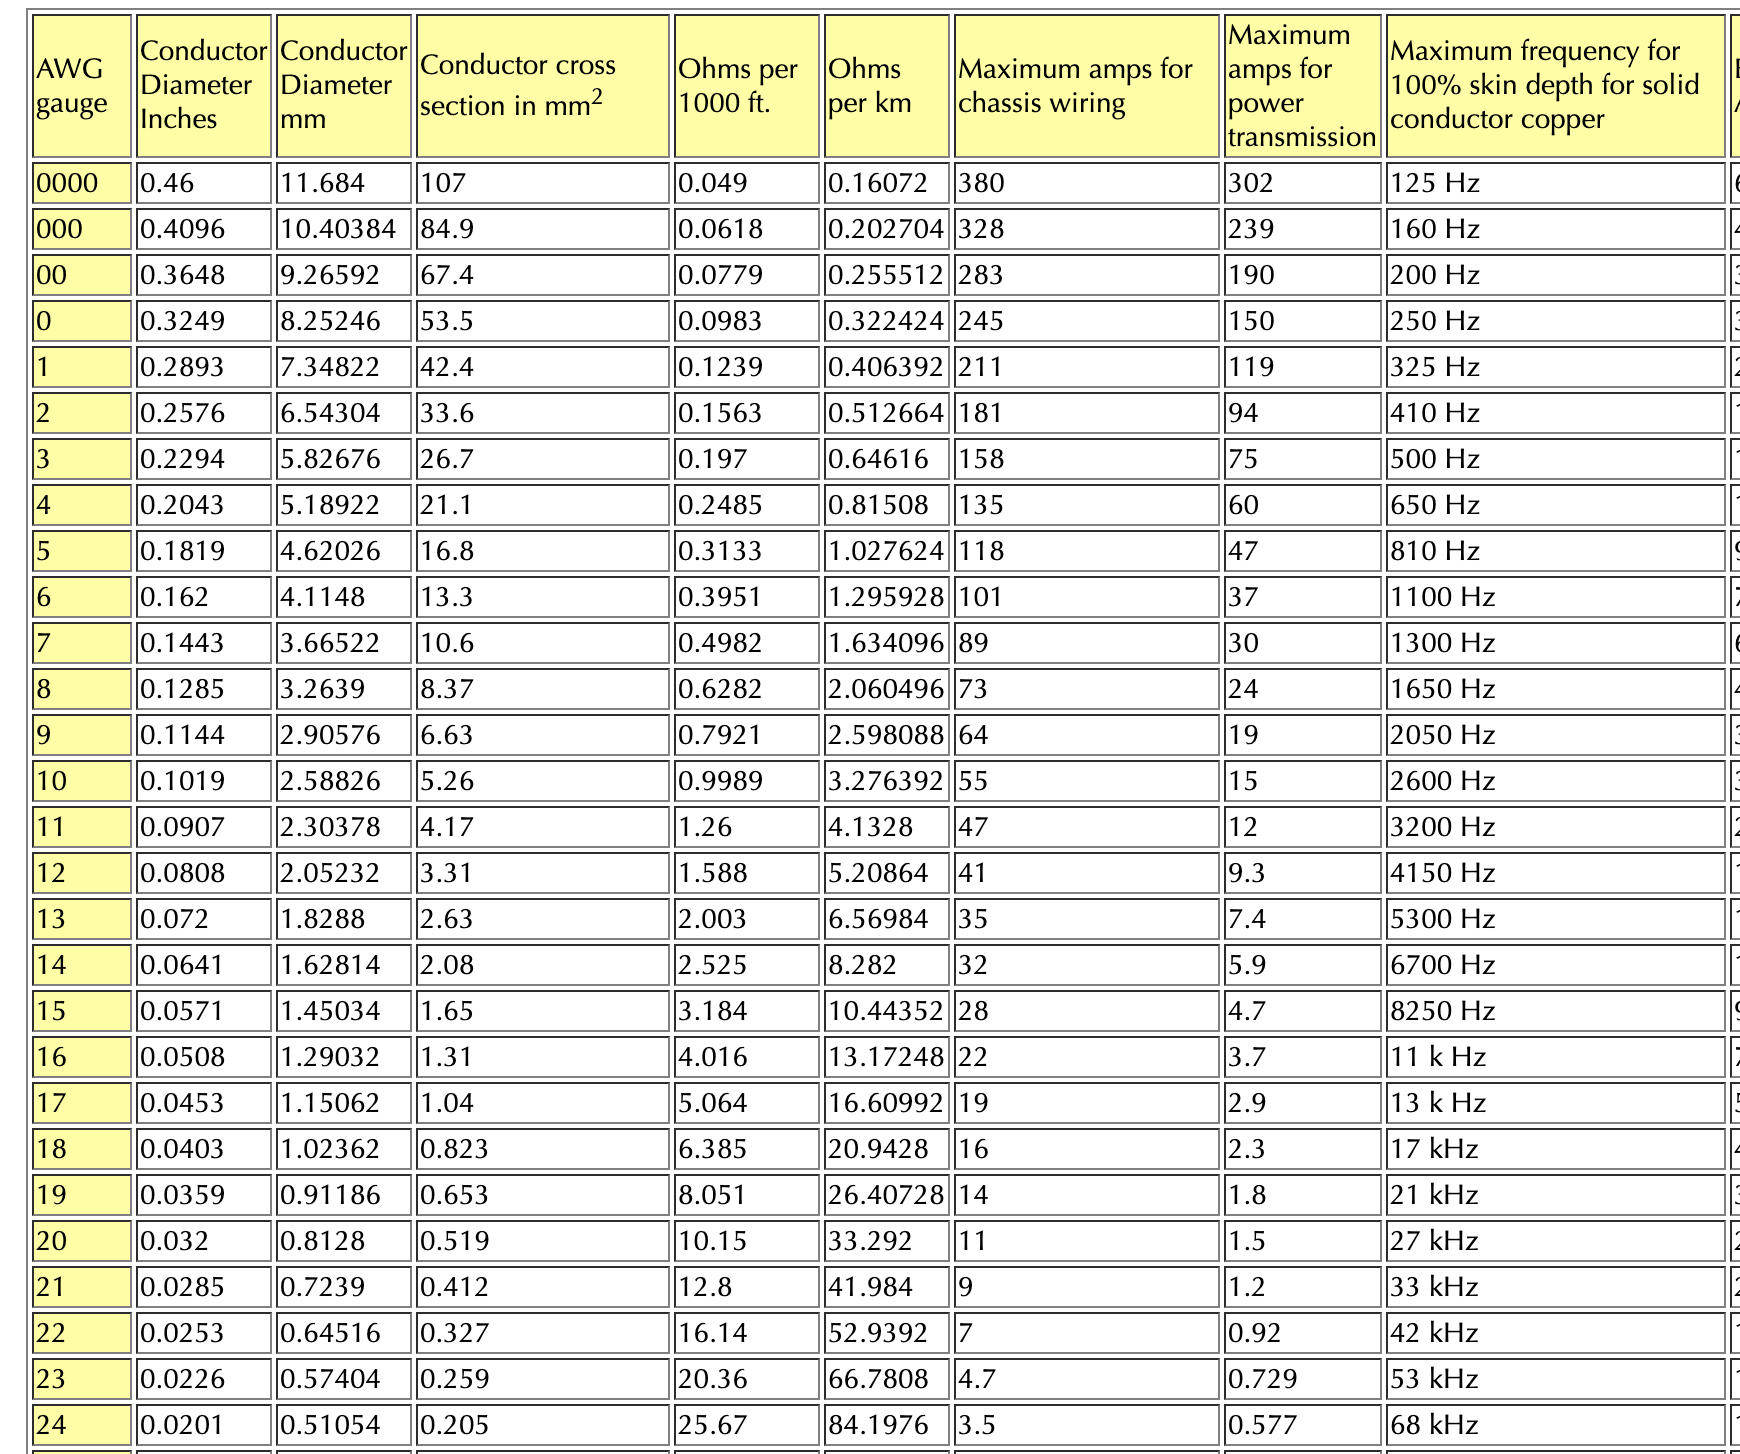
\includegraphics[scale=0.3]{kablo.png}
     \caption{Wire gauge chart.}
     \label{fig:my_label}
 \end{figure}
 \begin{gather*}
     I_{pri}^{rms}=4.52 A\\
     I_{sec}^{rms}=I_{ds}^{rms}\sqrt{\frac{1-D{max}}{D_{max}}}\frac{V_{RO}}{V_o+V_F}\\
     V_{RO}=\frac{D_{max}}{1-D_{max}}V_{in}^{min}\\
      I_{sec}^{rms}=6.67A\\
      \text{Choose} \: J=6 A/mm^2\\
      A_{pri}=\frac{4.52}{6}\approx0.76\\
      A_{sec}=\frac{6.67}{6}\approx1.11\\
      \text{Pick 3xAWG23 and 4xAWG22}\\
      k_u(fill \, factor)=\frac{3*0.259*30+4*0.327*20}{77.6}=\%64
 \end{gather*}

\begin{gather*}
    MLT=\pi *(E+F)/2=39.3285mm \tab \text{E and F are the core parameters shown in Datasheet.}\\
Length \:primary= 30*39.3285=11780 mm\\
Legth \: secondary= 20*39.3285=786.57mm\\
R_{pri}=(66.78*1.18*10^{-3})/3=0.0262 \Omega\\
R_{sec}=(52.9392*0.786*10^{-3})/4=0.0104\Omega
\end{gather*}

There is no need to calculate the AC resistances since skin effect is already considered during wire selection. In other words, it can be taken as same with the dc resistances by neglecting the proximity effect.
\begin{gather*}
    P_{cu}=I_{pri(rms)}^2*R_{pri}+ I_{sec(rms)}^2*R_{sec}=4.5222*0.0262+6.6732*0.0131=1.119W
\end{gather*}



 \subsection{Diode Selection}
 \begin{gather*}
     V_D=V_o+\frac{V_{in}^{max}(V_o+V_F)}{V_{RO}}\approx47V\\
     I_D^{rms}=I_{sec}^{rms}=6.67A
 \end{gather*}
 
 \subsection{Output Capacitor Selection}
 \begin{gather*}
     \Delta V_0=\frac{I_oD_{max}}{C_of_s}+\frac{I_{ds}^{peak}V_{RO}R_C}{V_o+V_F}\\
     R_C= 15m\Omega\\
     \Delta V_o \,\text{is desired \%4 which is equal to 0.6V deviation}\\ 
     \text{Let's make a conservative selection} \Delta V_o=0.35V
     \Delta V_o=\frac{4*0.492}{C_o*4*10^4}+\frac{8.2*24*0.015}{15.5}\\
     0.35=\frac{4.92*10^{-5}}{C_o}+0.19\\
     C_o=\frac{4.92*10^{-5}}{0.16}\\
     C_o\approx330\mu F\\
 \end{gather*}
 
 \subsection{RC-Snubber Design}

\begin{figure}[H]
    \centering
    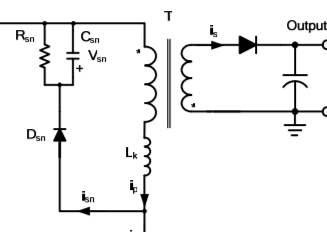
\includegraphics{f9.png}
    \caption{RCD snubber.}
    \label{fig:my_label}
\end{figure}

During the off time, additional voltage stress may occur on Mosfet (switch) due to leakage inductance of the
transformer and they may damage the Mosfet. Therefore, a RCD snubber has designed to reduce that extra stress on Mosfet, shown in Figure 8. The components of that circuit depends on the primary leakage inductance, so they may be changed after measuring the leak-
age inductance in practice. For theoretical calculations, leakage inductance is
taken as \%1 of the primary inductance.\\
When the Mosfet turns off, current on the leakage inductance starts to flow through the RCD snubber and it supress the voltage stress on that node due to ringing effect. To design RCD snubber, the steps are followed:
\begin{enumerate}
    \item Measure leakage inductance
    *Due to pandemic condition, we have used \%1 of the magnetizing inductance $L_m$.\\
    $L_{leakage}=L_m*0.01=0.7\mu H$\\
    \item Determine peak clamp voltage:
    \begin{gather*}
        P=\frac{1}{2}LI_{peak}^2f_s\\
        P=\frac{1}{2}*7*10^{-7}(6.5)^2*4*10^4\approx 0.6W\\
        V_f=70V \: V_x=70/3V\\
        P_{snubber}^{max}=0.6(1+\frac{V_f}{V_x})=2.4W\\
    \end{gather*}
    \item Selecting clamp resistor:
    \begin{gather*}
     R=\frac{2V_xT_s(V_f+V_x)}{LI_p^2}\\
    R=\frac{2*23.3*(93.3)}{7*10^{-7}*(6.5)^2*4*10^{-4}}\approx3.67k\Omega\\
    \end{gather*}
\end{enumerate}




\section{Compensator Design and Controller}
\subsection{Compensator Design}

To construct a compensator circuit for closed loop control, the transfer function of the circuit should be derived by using small-signal model of Flyback converter. In this process, super-position method has been used. Control-to-output transfer function of CCM Flyback is derived below:\\


In order to achieve the small signal model of the flyback converter; capacitor current, inductor voltage and input current equations should be derived for both ON and OFF states of the switch.

\begin{enumerate}
    \item Switch is OFF:
    \begin{figure}[H]
        \centering
        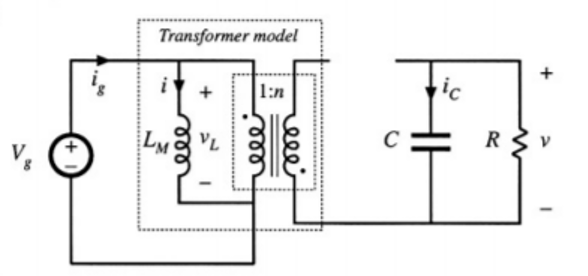
\includegraphics{SOFF.png}
        \label{fig:my_label}
    \end{figure}
    \begin{gather*}
        V_L=V_g\, i_c=-\frac{V}{R}\,i_g=I\\
    \end{gather*}
    
     \item Switch is ON:
    \begin{figure}[H]
        \centering
        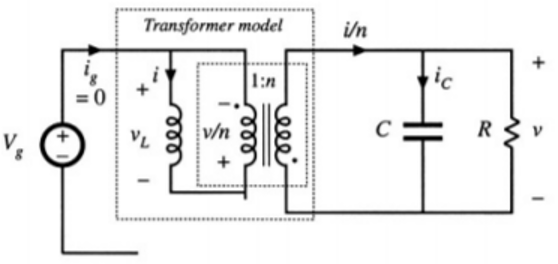
\includegraphics{SON.png}
        \label{fig:my_label}
    \end{figure}
    \begin{gather*}
        V_L=-\frac{V}{n}\: i_c=\frac{I}{n}-\frac{V}{R}\:i_g=0
    \end{gather*}
    
    
    Averaging and Linearizing:
    \begin{gather*}
        V_c=V \tab V_L=DV_g-\frac{D'V}{n}\\
        i_c=-\frac{DV}{R}+D'(-\frac{V}{R}+\frac{I}{n}) \tab i_g=DI\\
    \end{gather*}
    Considering AC perturbations following AC circuits are obtained.
    \item Inductor voltage:
    \begin{figure}[H]
        \centering
        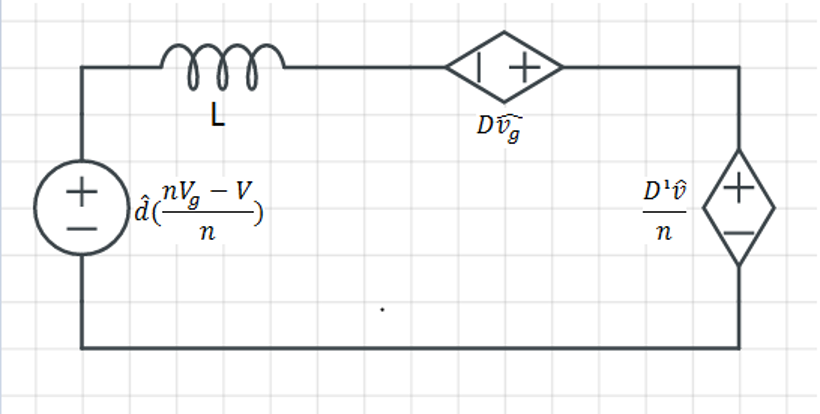
\includegraphics[scale=0.75]{x1.png}
        \label{fig:my_label}
    \end{figure}
    
    \begin{gather*}
        L\frac{d\tilde i_L}{dt}=D\tilde v_g+\tilde dV_g-\frac{D'\tilde v-\tilde dV}{n}=\tilde d (\frac{nV_g-V}{n})+D\tilde v_g-\frac{D'\tilde v}{n}\\
    \end{gather*}
    
    \item Capacitor current:
    \begin{figure}[H]
        \centering
        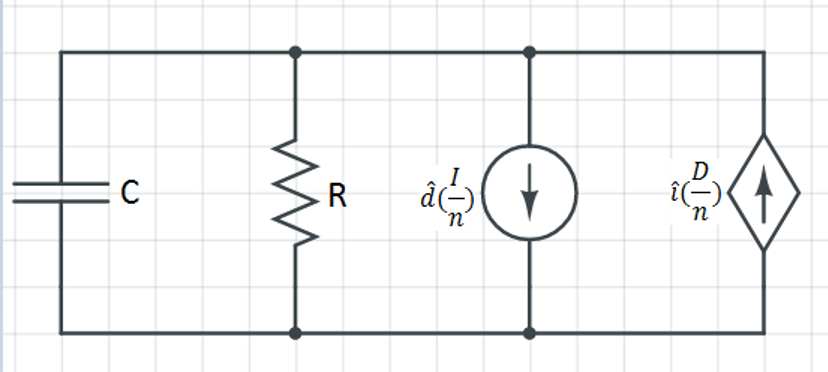
\includegraphics[scale=0.75]{x2.png}
        \label{fig:my_label}
    \end{figure}
    
    \begin{gather*}
        C\frac{d\tilde V}{dt}=-\frac{D\tilde v+\tilde d V}{R}-\frac{D'\tilde v}{R}+\frac{\tilde d V}{R}+\frac{D'\tilde i}{n}-\frac{\tilde d I}{n}\\
        =-\tilde d \frac{I}{n}-\frac{\tilde v}{R} +\tilde i \frac{D}{n}\\
    \end{gather*}
    
    \newpage
    \item Input current:
    \begin{figure}[H]
        \centering
        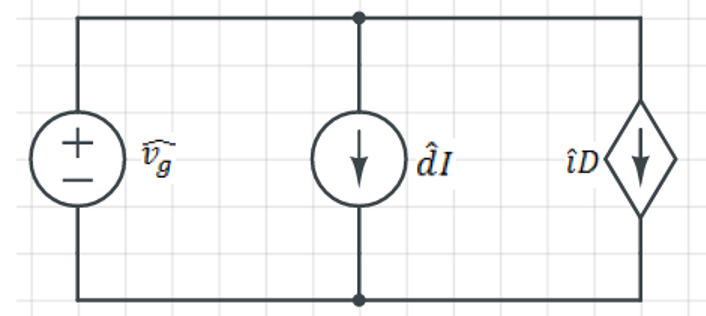
\includegraphics[scale=0.75]{x3.png}
        \label{fig:my_label}
    \end{figure}
    
    \begin{gather*}
       \tilde i_g =\tilde iD+\tilde d I\\
    \end{gather*}
    
   
\end{enumerate}
 

Adding these three circuits one after another will result with :\\
L: magnetizing inductor \tab I: inductor current\tab $R_on$:diode resistor\\
V:output voltage \tab $V_g$: input voltage
\begin{figure}[H]
    \centering
    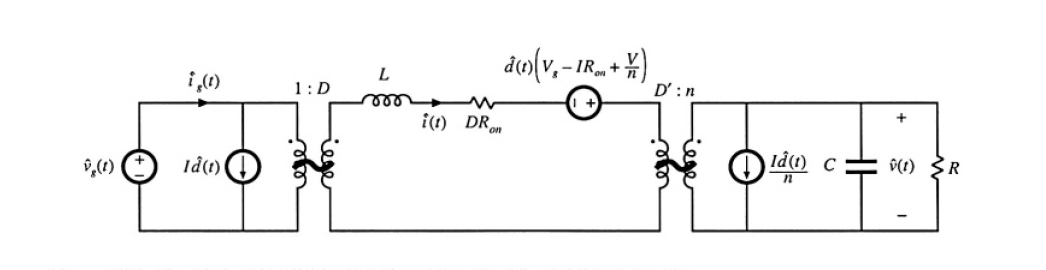
\includegraphics[scale=0.75]{Small-signal.png}
    \caption{Small-signal ac equivalent circuit model of Flyback converter.}
    \label{fig:my_label}
\end{figure}
\newpage
\begin{enumerate}

    \item Killing current source:
     \begin{figure}[H]
        \centering
        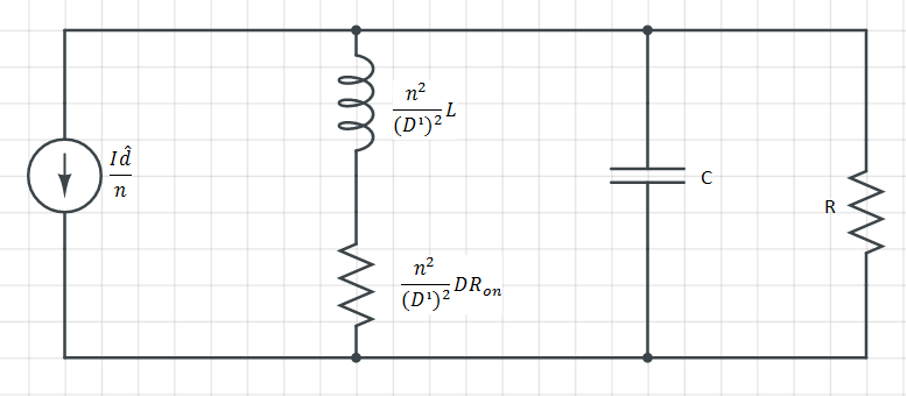
\includegraphics[scale=0.75]{x4.png}
        \label{fig:my_label}
    \end{figure}
    \begin{gather*}
        \frac{\tilde V}{\tilde d}=\frac{(nV_g-nIR_{on}+V)}{D'}*\frac{R\parallel\frac{1}{sC}}{(sL+DR_{on})\frac{n^2}{D'^2}+(R\parallel\frac{1}{sC})}\\
        \frac{\tilde V}{\tilde d}=\frac{(nV_g-nIR_{on}+V)D'R}{n^2(sL+DR_{on})(sCR+1)+D'^2R}\\
    \end{gather*}
    \item Killing voltage source ($R_{on}$ is ignored for ideal case):
     \begin{figure}[H]
        \centering
        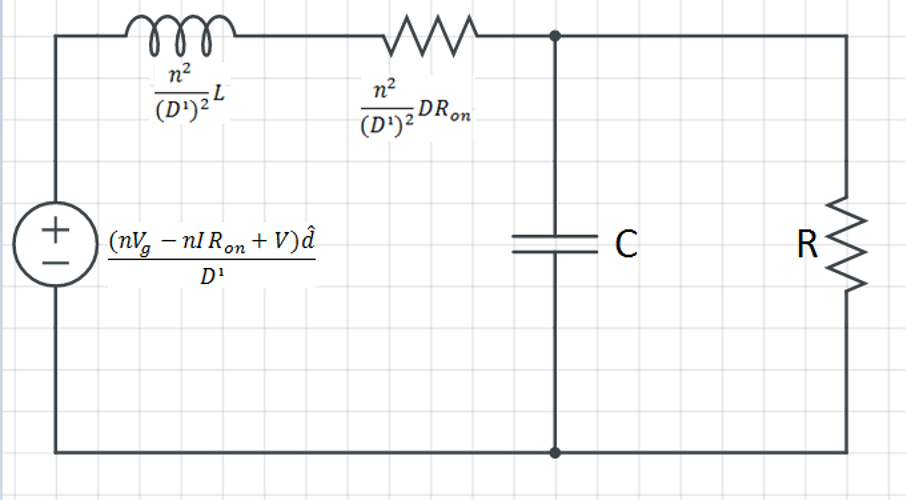
\includegraphics[scale=0.75]{x5.png}
        \label{fig:my_label}
    \end{figure}
    \begin{gather*}
        \frac{V(s)}{d(s)}=\frac{-I(sL)nR+D'R_nV_g+VD'R}{(sL+DR_{on})(sCR+1)n^2+RD'^2}\\
        I=\frac{I_s}{D'} \tab I_s=\frac{D}{D'}n\frac{V}{R}\\
        V=\frac{D}{D'}nV_g \tab I=\frac{D}{D'^2}n^2\frac{V_g}{R}\\
        \frac{V(s)}{d(s)}=\frac{(\frac{-D}{D'^2}n^3(sL)+D'R_n+DnR)V_g}{(sL)(sCR+1)n^2+RD'^2}\\
        \frac{V(s)}{d(s)}=\frac{nV_g(-\frac{D}{(1-D)^2}n^2(sL)+R)}{s^2n^2RLC+sL_n^2+R(1-D)^2}\\
        \frac{V(s)}{d(s)}=\frac{nV_g}{(1-D)^2}\frac{(-Dn^2sL+(1-D)^2)R}{s^2n^2RLC+sL_n^2+R(1-D)^2}\\
        =\frac{nV_g}{(1-D)^2}\frac{(1-\frac{s}{\frac{(1-D)^2}{Dn^2L}})}{(1+\frac{s}{\frac{(1-D)^2R}{L_m^2}}+\frac{s^2}{\frac{(1-D)^2}{n^2LC}})}\\
    \end{gather*}
\end{enumerate}
\begin{figure}[H]
    \centering
    \includegraphics[scale=0.2]{open loop direkt Flybackin(oscillator yok).jpg}
    \caption{Control-to-output transfer function bode plots of the designed Flyback converter .}
    \label{fig:my_label}
\end{figure}
    \begin{figure}[H]
    \centering
    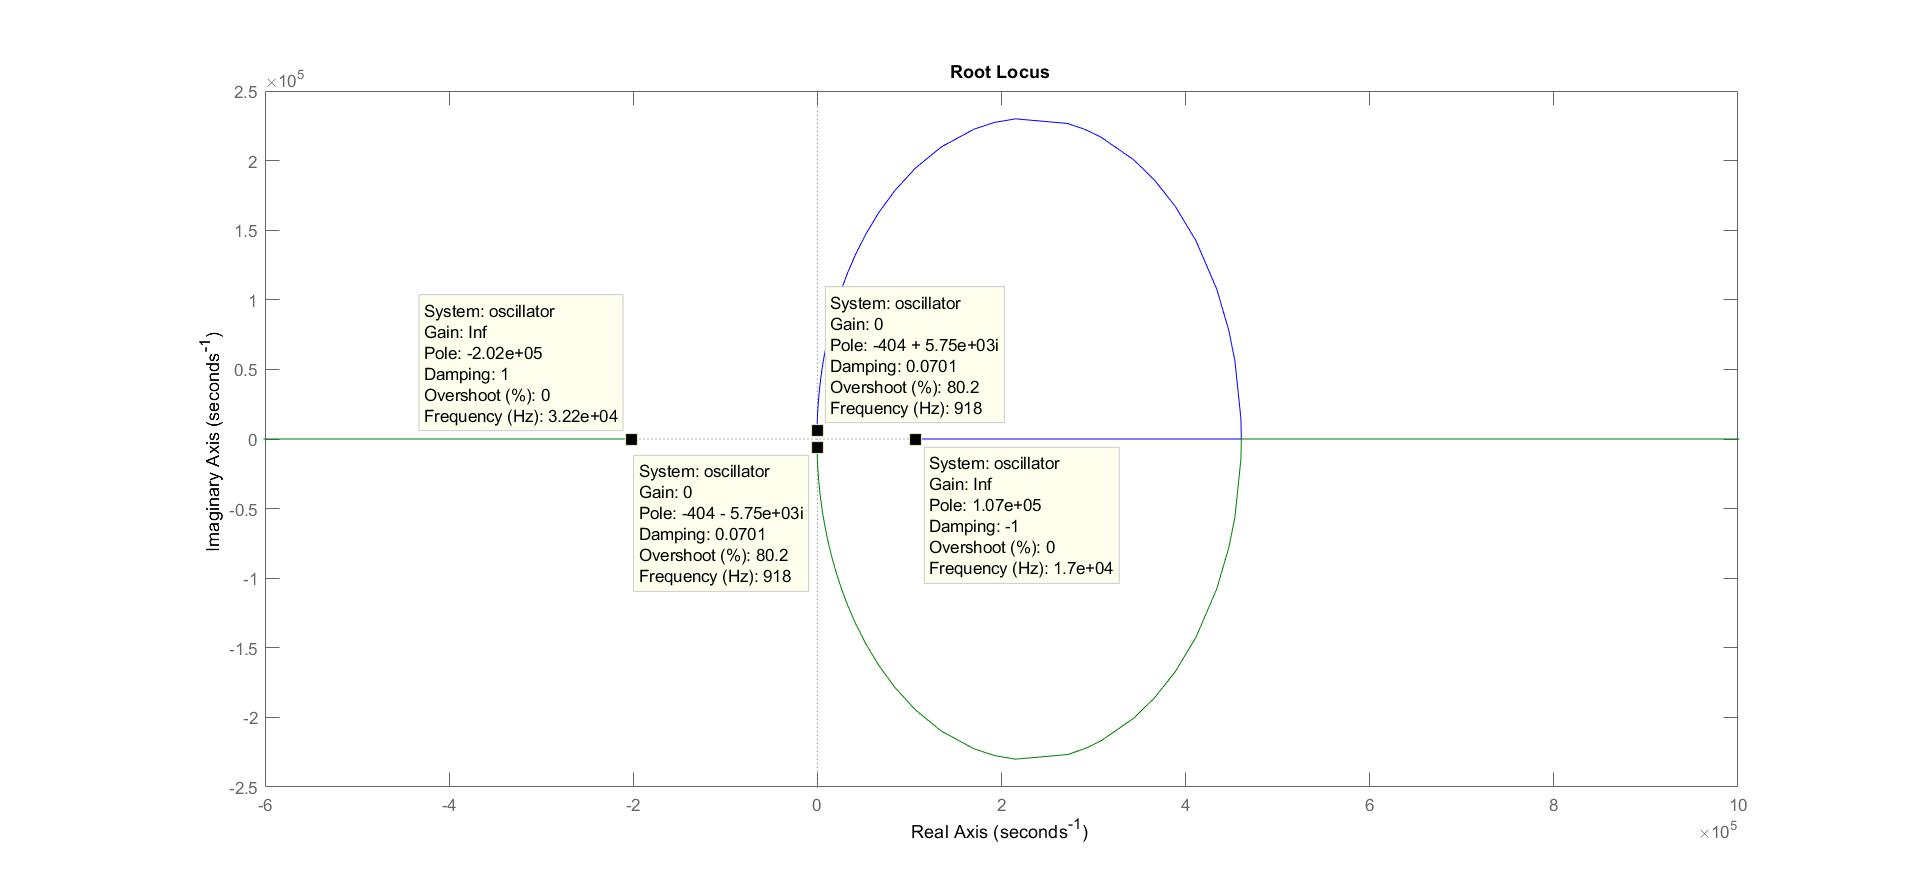
\includegraphics[scale=0.2]{pole zero locations detection with rlocus.jpg}
    \caption{Root locus of the designed Flyback converter's control-to-output transfer function.}
    \label{fig:my_label}
\end{figure}

The open-loop characteristic of our Flyback converter and the zero/pole locations of the control-to-output transfer function of it are illustrated in Figure 10 and 11. Without a compensator, the design is not stable which can be observed from both root loci and negative phase margin. To achieve a stable closed-loop system, at least $40^0-45^0$ phase margin is necessary. Moreover, ESR of the output capacitor is very important because it introduces an extra zero to system.
In this respect, a Type-3 error amplifier is designed and implemented by following steps: 

\begin{enumerate}
    \item Assume $V_{osc}^{peak}=1.8V$\\
    \item Select crossover frequency $\frac{f_{sw}}{10}<f_c<\frac{f_{sw}}{5}$\\
    Let's choose it $f_c=\frac{f_{sw}}{5}=8kHz.$\\
    \item Location of poles and zeros:
    \begin{gather*}
        f_{ESR}>\frac{f_{sw}}{2}>f_c>f_{LC} \tab \text{Type-3B}\\
        f_{LC}=918Hz\\
        \frac{f_{sw}}{2}=20kHz\\
        f_{ESR}=32.2kHz\\
        f_{RHPZ}=17kHz\\
        f_c=8kHz\\
    \end{gather*}
 \begin{figure}[H]
    \centering
    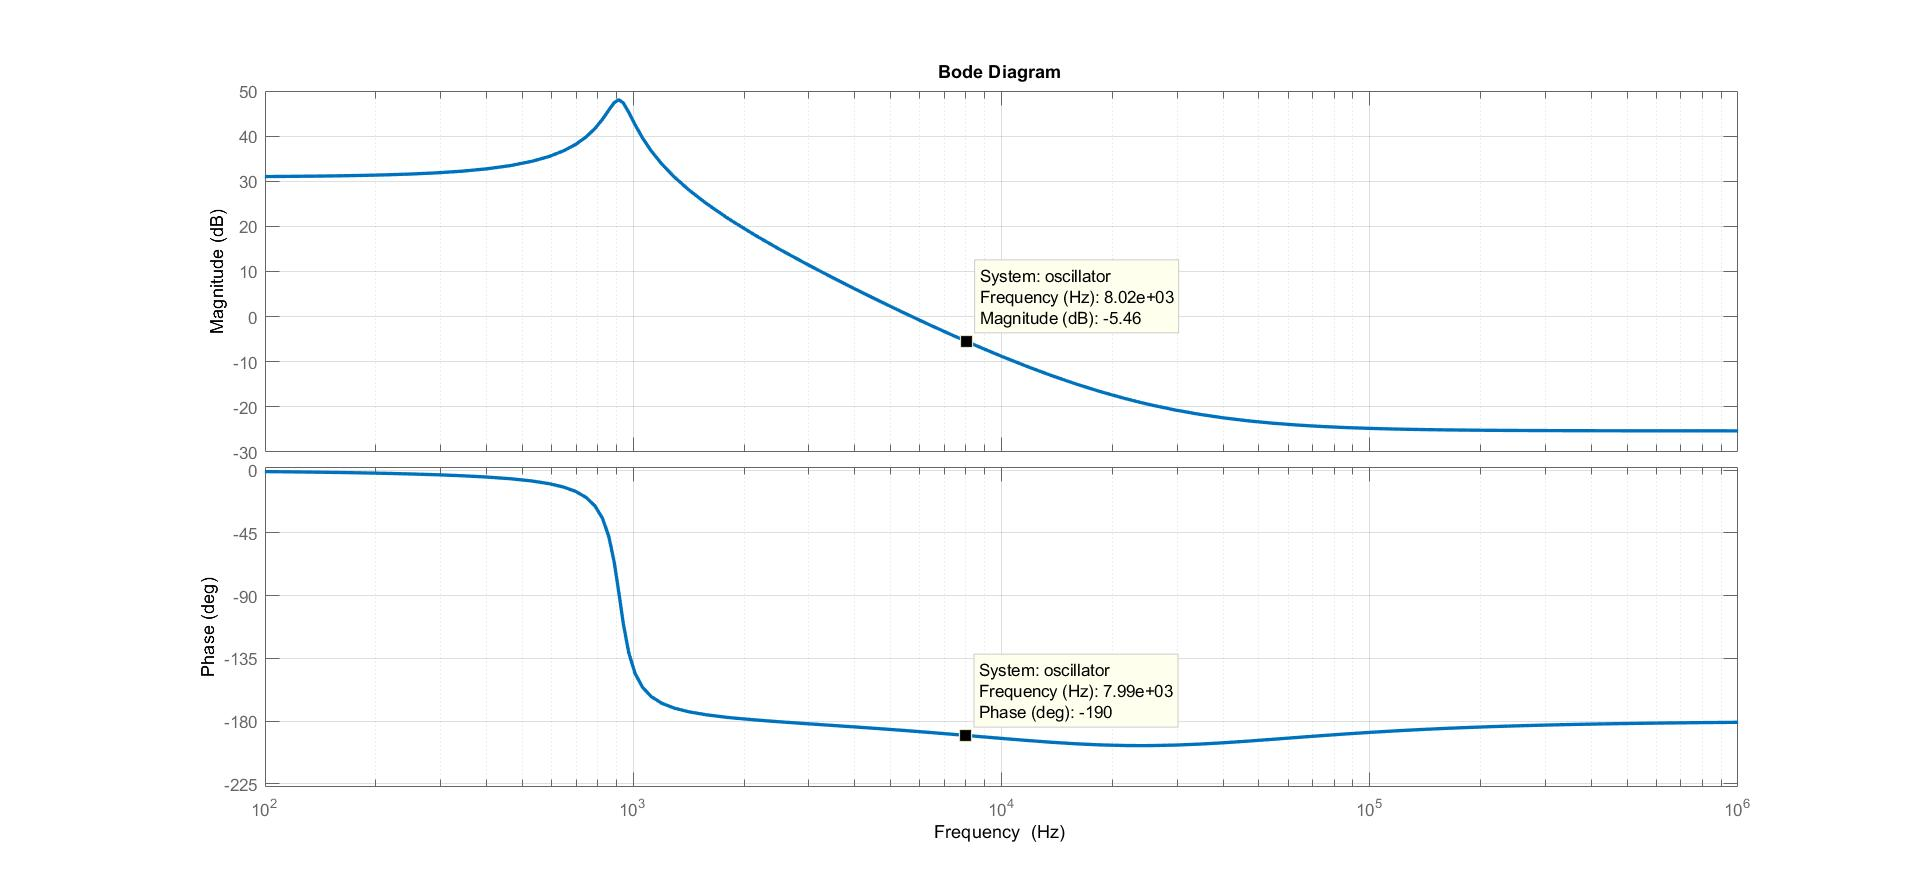
\includegraphics[scale=0.2]{phase and gain at crossover frequency of open loop system.jpg}
    \caption{Bode plot of control-to-output transfer function, marked $f_c$.}
    \label{fig:my_label}
\end{figure}
\item Determine needed phase and gain at $f_c$ from Figure 12:
\begin{gather*}
    \text{at $f_c=8kHz$:}\\
    phase=-190^0 \tab gain=-5.6dB\\
    \Theta_{compensator}=45-(-190)=235^0\\
    Gain_{compensator}=5.4dB(1.862)
\end{gather*}
\item Derive the Type-3B compensator' components by using K-method, as illustrated in Figure 13:
 \begin{figure}[H]
    \centering
    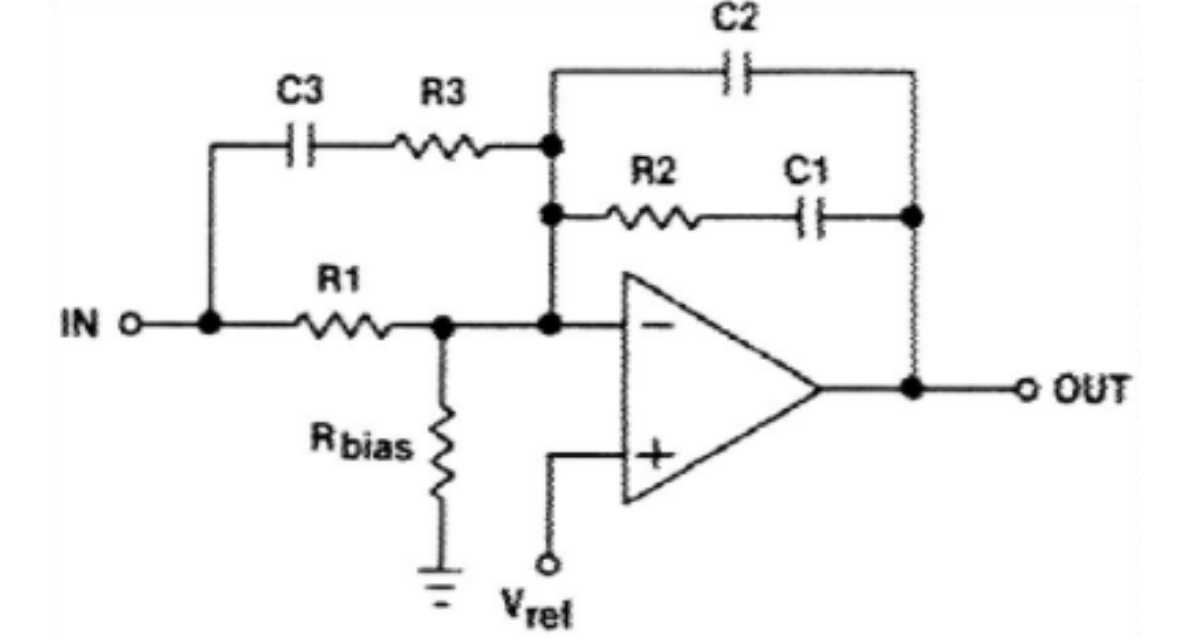
\includegraphics[scale=0.5]{Type-3.png}
    \caption{Schematic of the designed Type-3 compensator.}
    \label{fig:my_label}
\end{figure}

\begin{gather*}
    \text{Start with} \: R_1=1k\Omega\\
    R_2=\frac{|G(jw_{c})|}{\sqrt{K}}=\frac{1.862*1000}{\sqrt{42.21}}=286\approx 270\Omega\\
    C_1=\frac{\sqrt{K}}{w_cR_2}=\frac{\sqrt{42.21}}{2\pi*8000*270}=479\approx470\mu F\\
    C_2= \frac{1}{w_cR_2\sqrt{K}}\approx10nF\\
    C_3=\frac{\sqrt{K}}{w_cR_1}\approx130nF\\
    R_3=\frac{1}{w_c\sqrt{K}C_3}\approx30\Omega\\
    V_{ref}=V_{out}\frac{R_{bias}}{R_{bias}+R_1}\\
    2.5=15*\frac{R_{bias}}{R_{bias}+1000}\\
    R_{bias}=200\Omega\\
\end{gather*}
\item Derive transfer function of the compensator: 
\begin{gather*}
    TF=-\frac{R_1+R_3}{R_1R_3C_2}*\frac{(s+\frac{1}{R_2C_1})(s+\frac{1}{(R_1+R_3)C_3})}{s(s+\frac{C_1+C_2}{R_2C_1C_2})(s+\frac{1}{R_3C_3})}\\
    =-(3.43*10^6)*\frac{s^2+17.58*10^3s+76.5*10^6}{s^3+7.11*10^5s^2+12.6*10^10s}\\
\end{gather*}

\end{enumerate}


\begin{figure}[H]
    \centering
    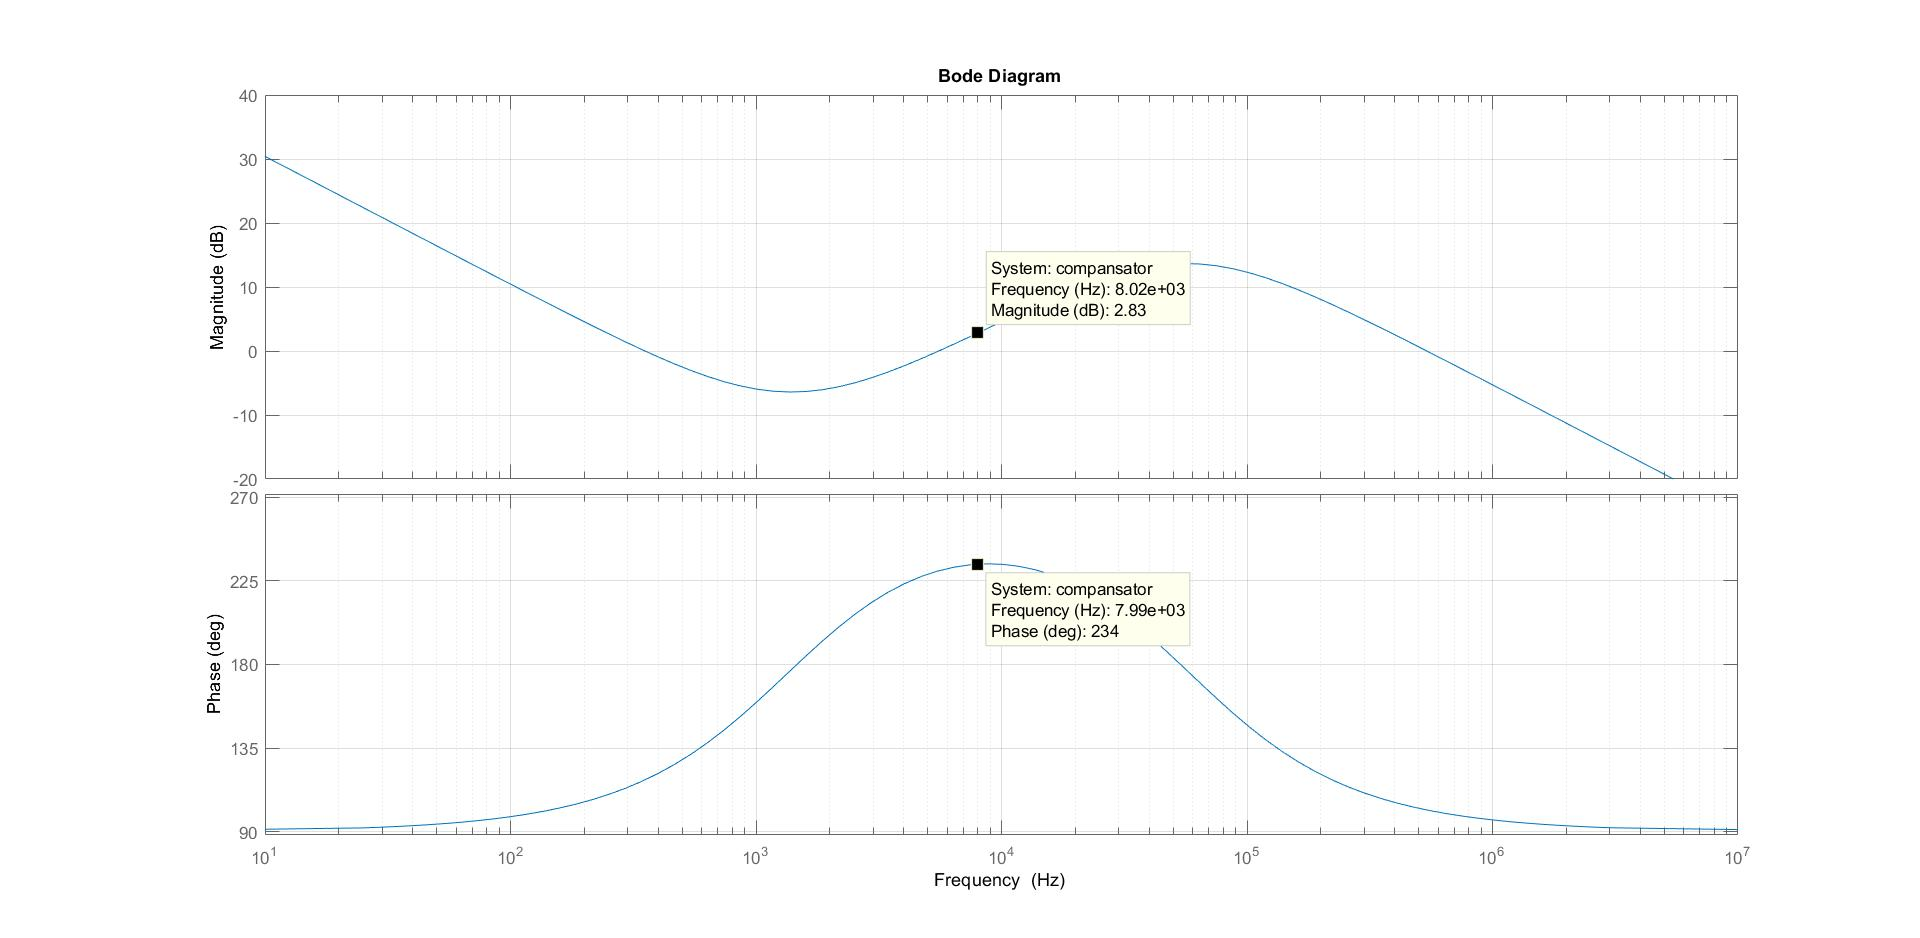
\includegraphics[scale=0.2]{compansator.jpg}
    \caption{Bode plot of the designed Type-3B compensator.}
    \label{fig:my_label}
\end{figure}
\begin{figure}[H]
    \centering
    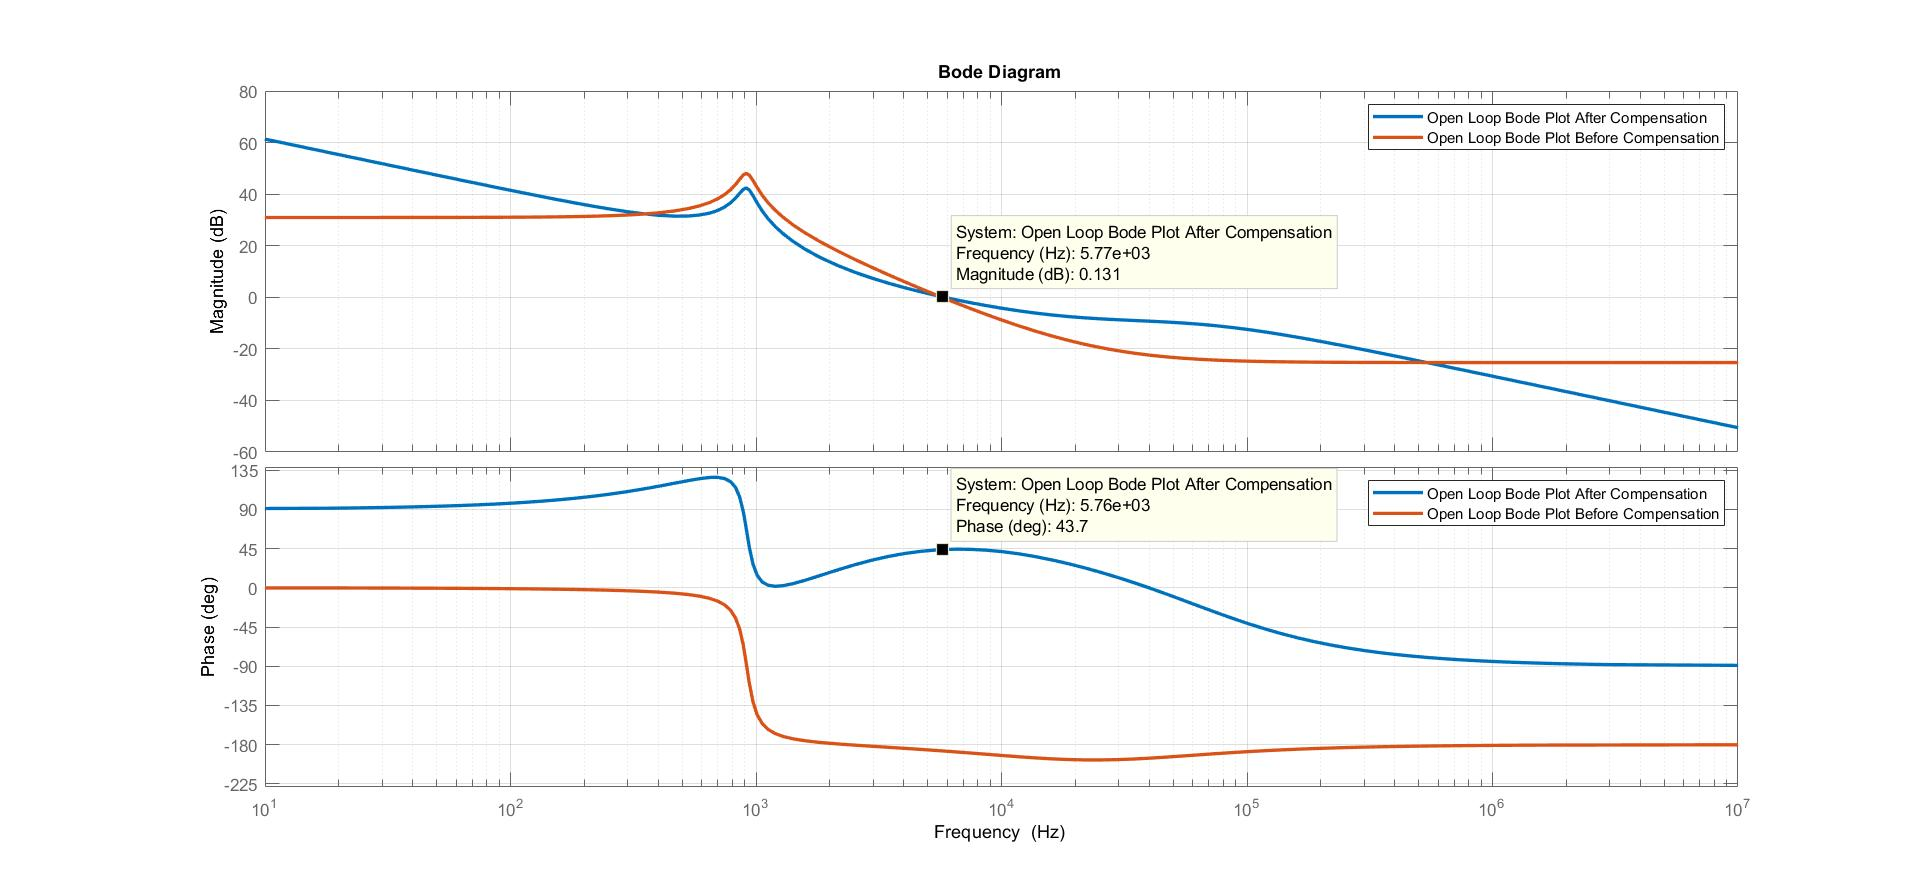
\includegraphics[scale=0.2]{after compensation.jpg}
    \caption{Bode plot of the Flyback converter with compensator.}
    \label{fig:my_label}
\end{figure}

With the designed Type-3B compensator, our system achieved $\Phi_{margin}=43.7^o$, which ensures the system stability, and  almost the desired crossover frequency, can be seen in Figure 14 and 15. The error of desired crossover frequency is the result of available components constrain. 













\subsection{Choosing Controller}
PWM Controller:\\
In order to make regulation for the output voltage, we need a some kind of feedback to some reference value, For that purpose, instead of using opamps to realize error amplifier, we have used “LT1246” PWM modulator. It has a wide range of oscillator frequency including the one that we have choose for the implementation which is 40kHz.
\begin{figure}[H]
    \centering
    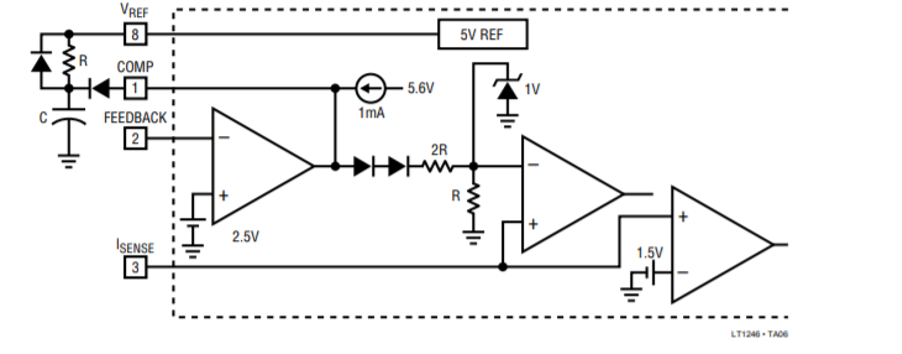
\includegraphics{IC.png}
    \caption{Error amplifier of the Lt1246.}
    \label{fig:my_label}
\end{figure}

It has its own internal error amplifier, which has a reference voltage of 2.5 Volt, therefore, in order to regulate 15 volt output voltage, we need to divide that value to be equal to 2.5 volt by creating voltage divider network. Also it has a “RT/CT” pin that can be connected to an “RC” circuit to adjusting its ramp waveform frequency.





\section{Efficiency and Thermal Analysis}
In power supply design, the electrical efficiency of the overall circuit and the junction temperature of semiconductor devices, which handle the conversion of power to a usable form, are very important points of design process.\\
MOSFET, diode and transformer losses are main elements of the scope of our thermal design.
Temperature of these components directly effect the performance of overall system, so we need to deal with it. To achieve better performance and thermal design, the thermal equivalent model is used, as illustrated in Figure 17 and 18.
\begin{figure}[H]
    \centering
    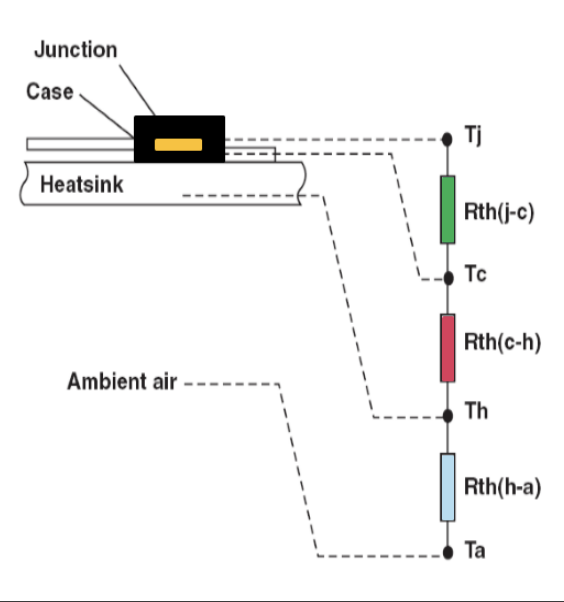
\includegraphics[scale=0.5]{thermal.png}
    \caption{Thermal equivalent model of a semiconductor.}
    \label{fig:my_label}
\end{figure}


\begin{figure}[H]
    \centering
    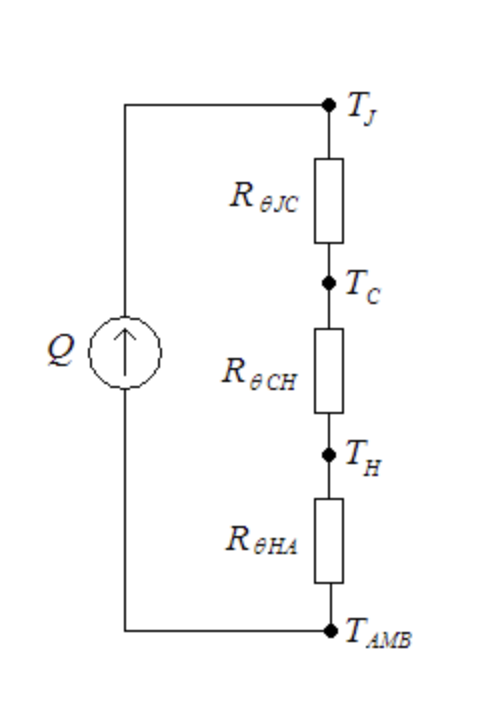
\includegraphics[scale=0.5]{thermal2.png}
    \caption{Electrical equivalent model of thermal model.}
    \label{fig:my_label}
\end{figure}
\newpage

According to these models, two heat sinks were implemented to PCB design for Mosfet and secondary side diode. 
\subsection{Mosfet Heatsink }
Conduction and switching losses are two main components of Mosfet' losses which should be taken into account for heat sink selection. The characteristic of thermal resistance of Mosfet and operating temperature interval were found in datasheet.In Figure 18, current source represents dissipated total power on the semiconductor and can be derived for Mosfet  as below: 
\begin{gather*}
    P_{tot}=P_{conduction}+P_{sw}\\
    P_{conduction}=I_{ds, rms}^2R_{ds,on}\\
    =(4.5)^2*0.15\approx3.04W\\
\end{gather*}
$R_{ds,on}$ depends on temperature, as seen in Figure 19, and operating junction temperature is chosen  90^0.

\begin{figure}[H]
    \centering
    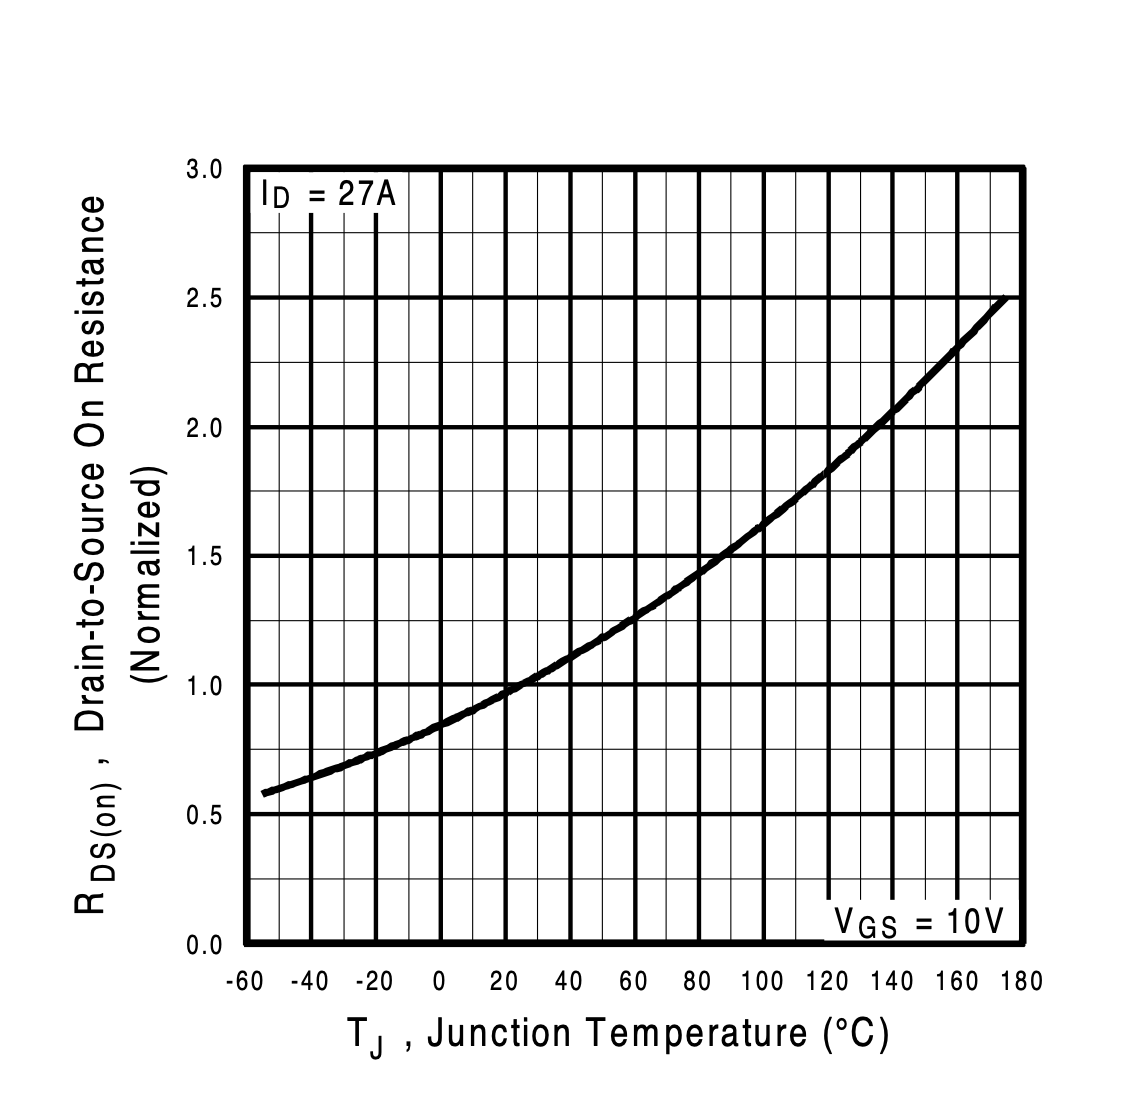
\includegraphics[scale=0.4]{Rds.png}
    \caption{$R_{ds}$ vs temperature characteristic of IRF540N.}
    \label{fig:my_label}
\end{figure}

\begin{gather*}
    P_{sw}=\frac{1}{2}(V_{ds}^{max}I_{ds}^{peak})t_ff_s\\
    =\frac{1}{2}*(48*8.5)*33*10^{-9}*4*10^4\approx0.27W\\
\end{gather*}

\begin{figure}[H]
    \centering
    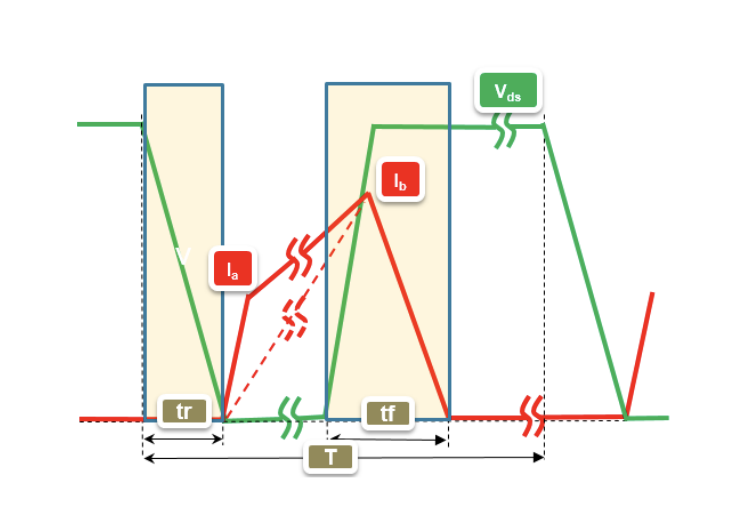
\includegraphics[scale=0.6]{sw.png}
    \caption{Inductive load switching.}
    \label{fig:my_label}
\end{figure}
\begin{gather*}
    P_{tot}=3.04+0.27=3.31W\\
    R_{j-c}=1.1 C^0/W \tab   R_{c-h}=0.5 C^0/W\\
    T_{junction}-T_{ambient}= P_{tot}*( R_{j-c}+R_{c-h}+R_{heatsink})\\
    (90^0-25^0)=3.31W*(1.6+R_{heatsink})\\
    R_{heatsink}=18C^0/W \\
\end{gather*}
As seen in Figure 21, HSE-B20250-040H is chosen for perfect fit and desired thermal resistance at operating point. It is TO-220 package heatsink which directly fit our Mosfet with same package.

\begin{figure}[H]
    \centering
    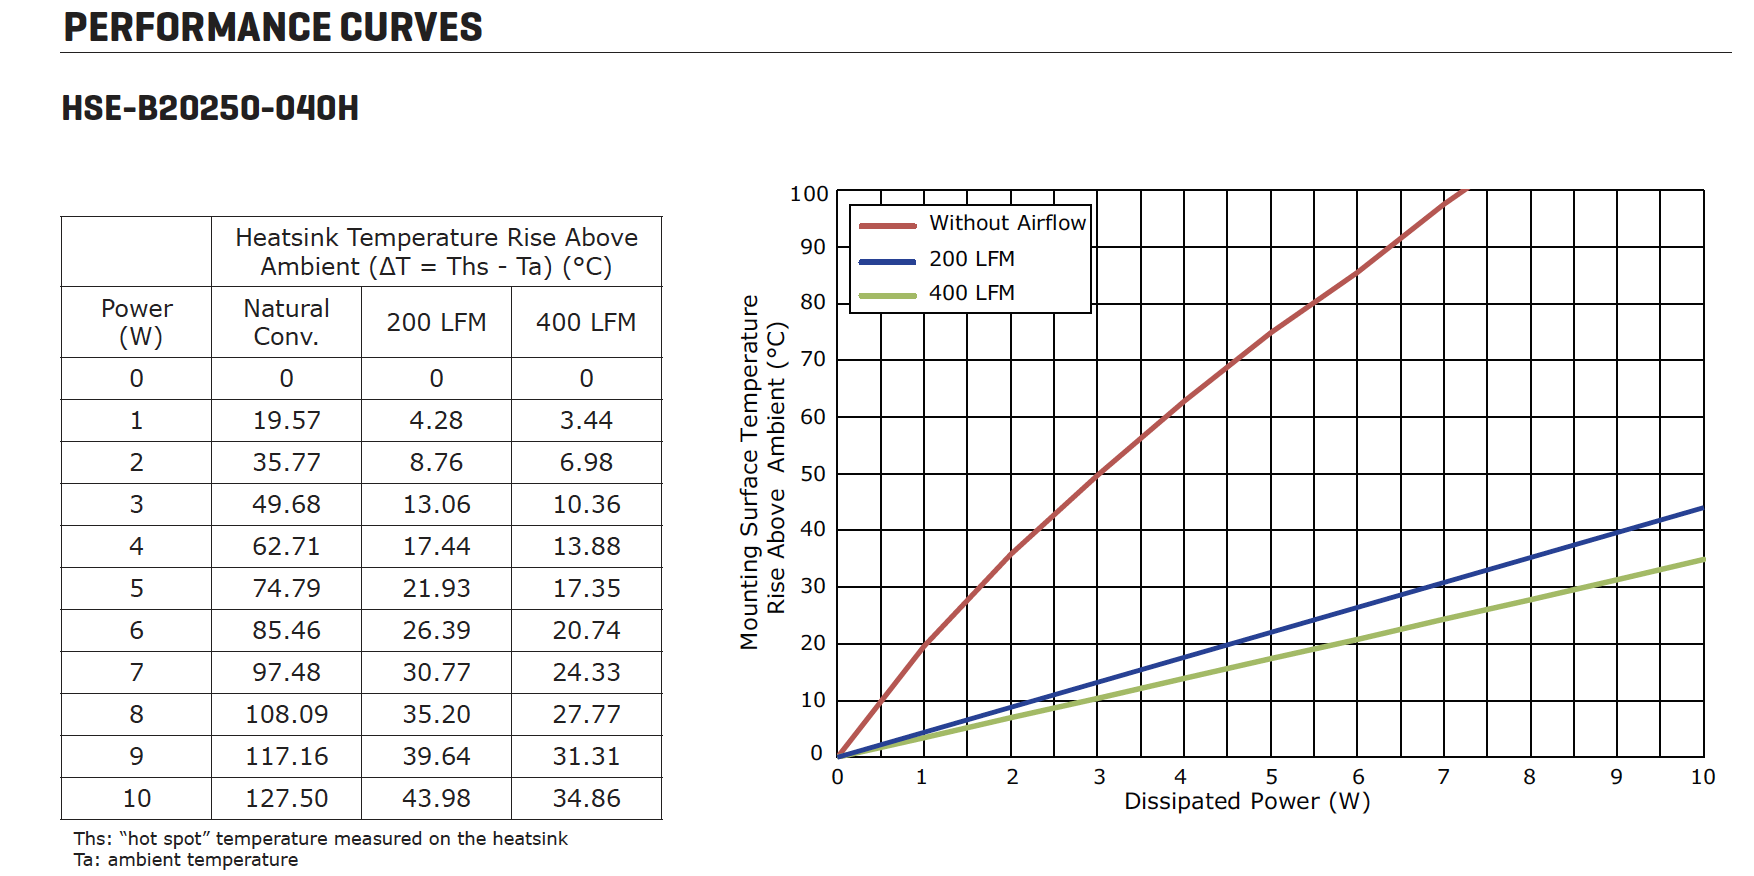
\includegraphics[scale=0.4]{heatsnk.png}
    \caption{HSE-B20250-040H performance curve.}
    \label{fig:my_label}
\end{figure}

\subsection{Diode Heatsink}
To find the correct heatsink same procedure and models has followed as Mosfet. The diode can operate maximum $150^0$ and we want to operate at $100^0$.
\begin{gather*}
    I_D\approx I_o=4A\tab V_D=0.47V \tab R_{on}=0.0133\Omega\\ 
    P_D=I_D*V_D+I^2R_{on}=2.12W\\
     R_{j-c}=1.5 C^0/W \\
     T_{junction}-T_{ambient}= P_{tot}*( R_{j-c}+R_{heatsink})\\
     \frac{75}{2.12}-1.5=R_{heatsink}\\
     =33.87 C^0/W \\
\end{gather*}

As seen in Figure 22, HSS-B20-0635H is chosen for perfect fit and desired thermal resistance at operating point. It is TO-220 package heatsink which directly fit our diode with same package.
\begin{figure}[H]
    \centering
    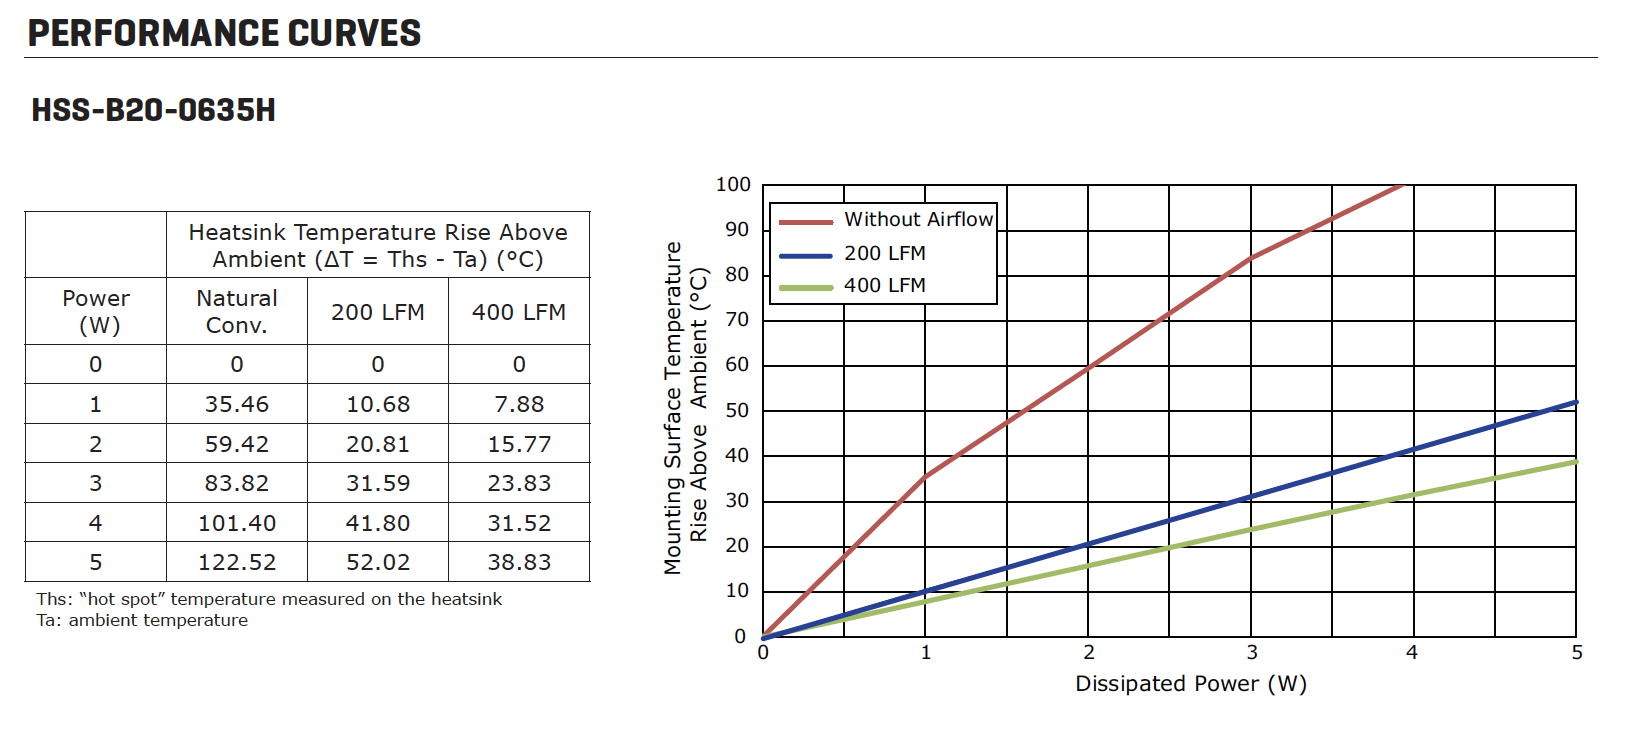
\includegraphics[scale=0.4]{Ekran Resmi 2020-06-25 05.08.14.png}
    \caption{HSS-B20-0635H performance curve.}
    \label{fig:my_label}
\end{figure}


\subsection{Transformer Losses}

\begin{gather*}
      P_{core}=568.8 mW/cm^3\\
    \text{Volume of selected core=}1.87 cm^3\\
    \text{Therefore core loss=}568.8*1.87=1.063W\\
     P_{cu}=I_{pri(rms)}^2*R_{pri}+ I_{sec(rms)}^2*R_{sec}=4.5222*0.0262+6.6732*0.0131=1.119W\\
     P_{transformer}=2.27W\\
 \end{gather*}



\section{PCB Design}
    A printed circuit board (PCB) mechanically supports and electrically connects electrical or electronic components using conductive tracks, pads and other features etched from one or more sheet layers of copper laminated onto and/or between sheet layers of a non-conductive substrate. Components are generally soldered onto the PCB to both electrically connect and mechanically fasten them to it.\\

	After the introduction, we are starting to mention about the process, challenges and solution of these challenges in flyback PCB design. 
	
	In this project, we have used Kicad pcb design tool to implement the design. Firstly all of the schematic of the circuit is implement by using the symbols. This process is important because we will next generate a netlist from these connections and later on, we will import this netlist in the PCB design layout. 

\begin{figure}[H]
    \centering
    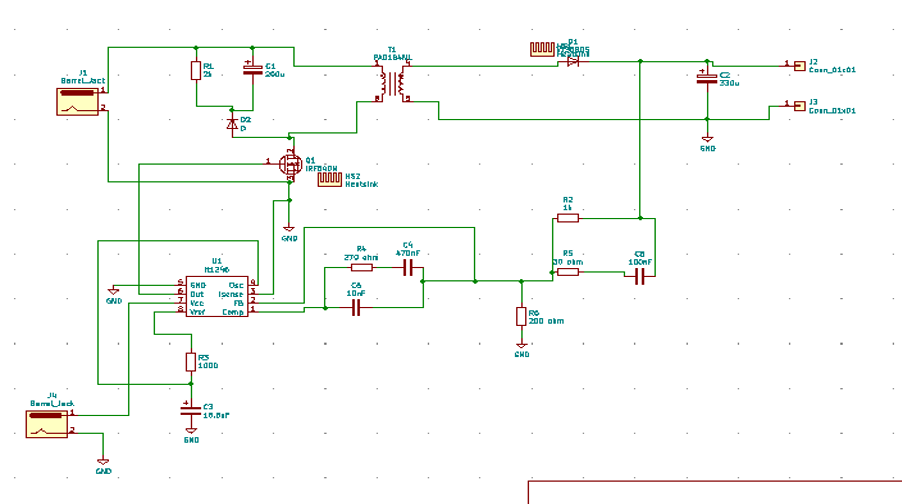
\includegraphics[scale=0.8]{PCB1.png}
    \caption{Schematic of the Flyback circuit.}
    \label{fig:my_label}
\end{figure}

As seen in Figure 23, all the connections between the components are done however, although it can not be understood from the figure, we have faced with several challenges in the implementation of this process because there isn’t any LT1246 symbol in the Kicad libraries thus, we had to make it ourselves, for that purpose, Symbol editor tool of the kicad is utilized to create that symbol because we have the data sheet and we know how many pins that we need to create that block.

\begin{figure}[H]
    \centering
    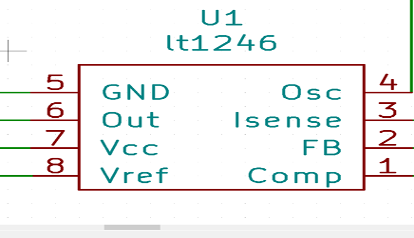
\includegraphics[scale=0.9]{PCB2.png}
    \caption{Symbol of the “LT1246” Controller IC.}
    \label{fig:my_label}
\end{figure}
After implementing the missing component symbol, placing resistor and capacitor symbols are straight forward. Therefore, in the next step, after completing the connections of the symbols, in the same page, we have started to assign footprints to symbols. And since, we have chosen nearly all of the components from digikey, this process was also straight forward but in order to assign a footprint to “Controller IC” we need to check its datasheet because there was not recommended assignment for that component.

\begin{figure}[H]
    \centering
    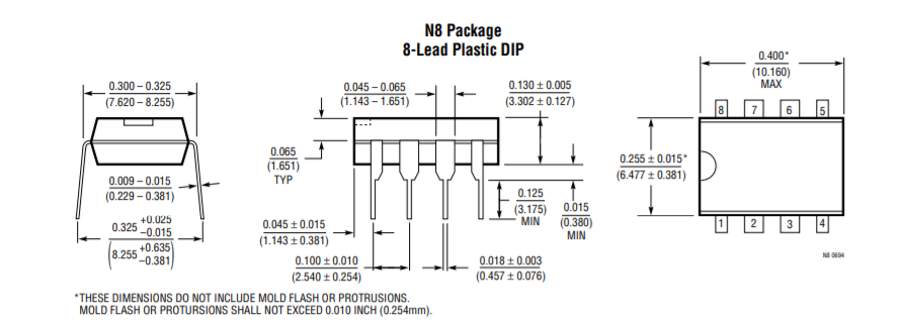
\includegraphics[scale=0.8]{PCB3.png}
    \caption{Package information of Lt1246.}
    \label{fig:my_label}
\end{figure}


In datasheet of that component, we have the package information and its package is common THT SO-DIP-8 package which can be seen for the most of the opamps, therefore it was available in the Kicad footprint library and it was assigned to that footprint.

After assigning of footprints, we have run the “electric rules checker” tool to see whether we can have any connection problems, after observing the checker, we have generated a netlist to export in to “layout” page.


In the second step, we were working on “PCB Layout” page to adjusting main PCB design, in that page we have created several types of tracks for the connection of the components in terms of how much current that these tracks will carry. In order to evaluate these track widths 
we have used “PCB track width calculator” webpage.




\begin{figure}[H]
    \centering
    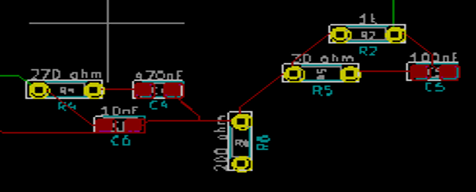
\includegraphics[scale=0.9]{PCB4.png}
    \caption{A view from the PCB layout page.}
    \label{fig:my_label}
\end{figure}

\begin{figure}[H]
    \centering
    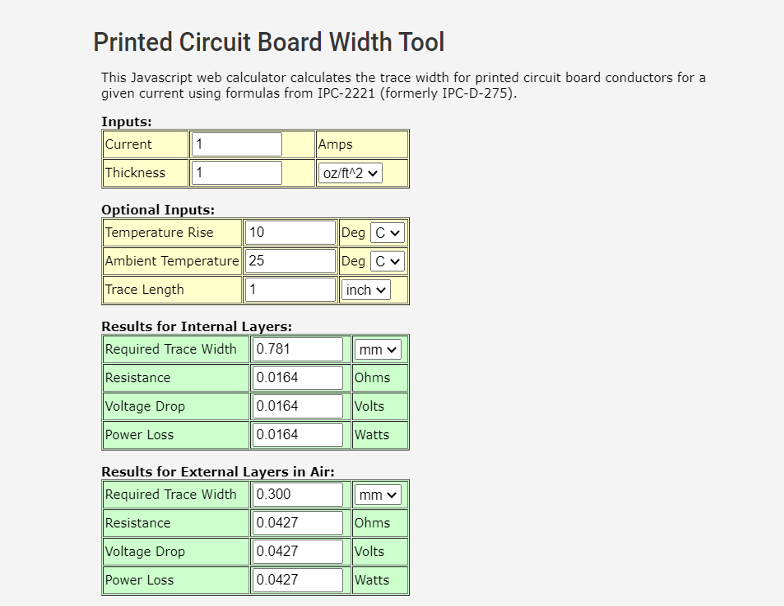
\includegraphics[scale=0.9]{PCB5.png}
    \caption{Captured when the controller output to gate  connection width calculated.}
    \label{fig:my_label}
\end{figure}

After calculating the track widths of all the connections, footprints are connected to each other. However, since the implementation of PCB design requires back and front copper layers, we have utilized from this process in several ways. For example since it is hard to jump a connection on another one in the PCB, we have used “back copper” layer for some connections to avoid wrong nodes and connections.
\begin{figure}[H]
    \centering
    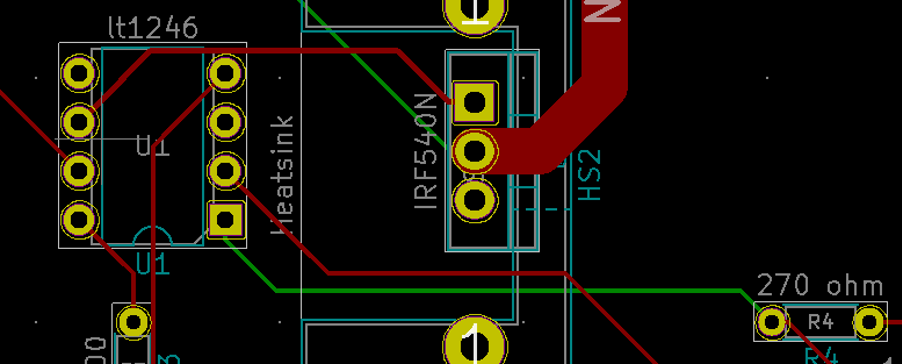
\includegraphics[scale=0.9]{PCB6.png}
    \caption{Illustration of back and front copper traces.}
    \label{fig:my_label}
\end{figure}
After checking the design warning and mistakes which is created by “design rules checker”, finally, we have connected all the grounds of the circuits by using front and copper layers. so, the layout process is completed.


\begin{figure}[H]
    \centering
    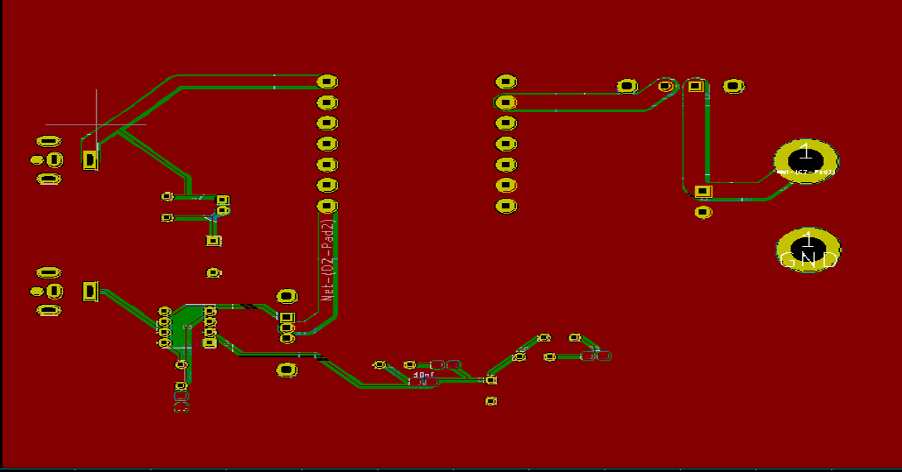
\includegraphics[scale=0.9]{PCB7.png}
    \caption{Final version of the PCB layout page. }
    \label{fig:my_label}
\end{figure}



After we have created all the layers inside the “Flyback” converter, next process is producing “gerber files” to make the PCB ready to be produced and it can be done using “plot” button of the PCB layout page and following several straightforward steps.


\begin{figure}[H]
    \centering
    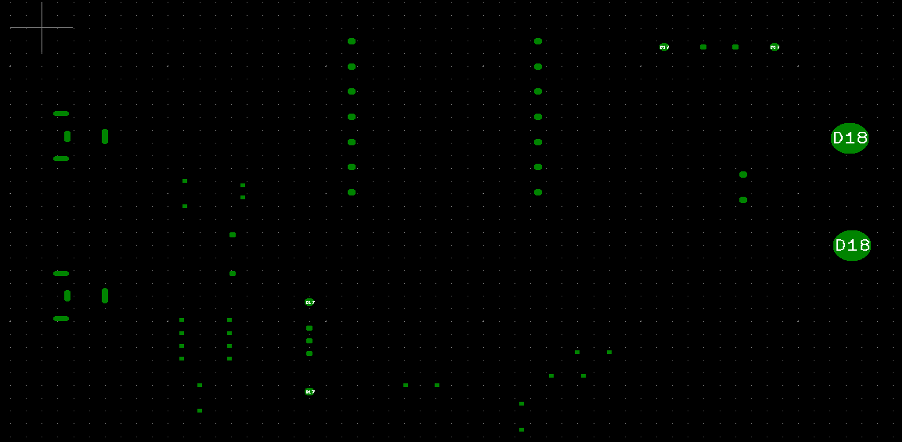
\includegraphics[scale=0.9]{PCB8.png}
    \caption{Opening “gerb view of drill files”. }
    \label{fig:my_label}
\end{figure}
Finally, we have taken a quote from the given website. (Bill of materials is on the github)


\begin{figure}[H]
    \centering
    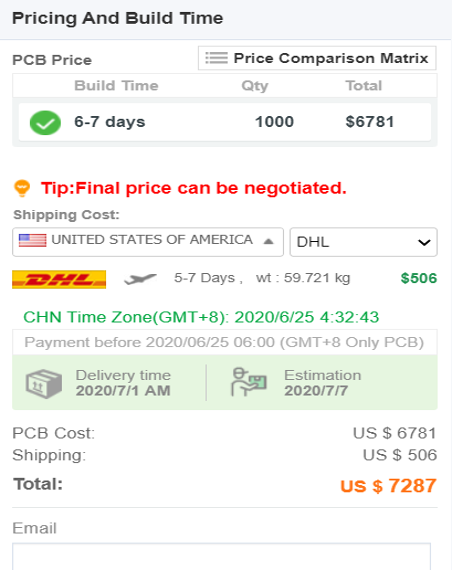
\includegraphics[scale=0.9]{PCB9.png}
    \label{fig:my_label}
\end{figure}


\subsection{3D Views of Design}

\begin{figure}[H]
    \centering
    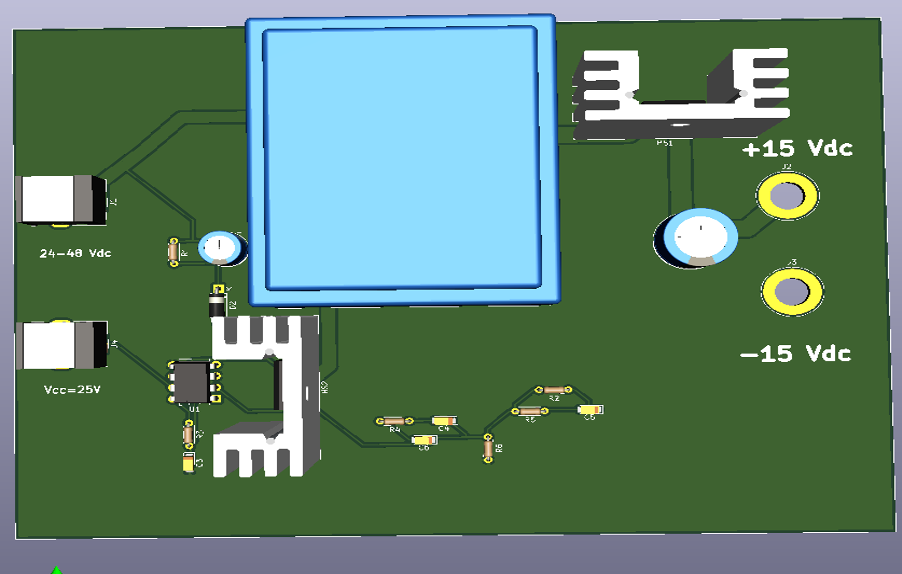
\includegraphics[scale=0.8]{PCB10.png}
    \caption{Top view of the circuit. }
    \label{fig:my_label}
\end{figure}

\begin{figure}[H]
    \centering
    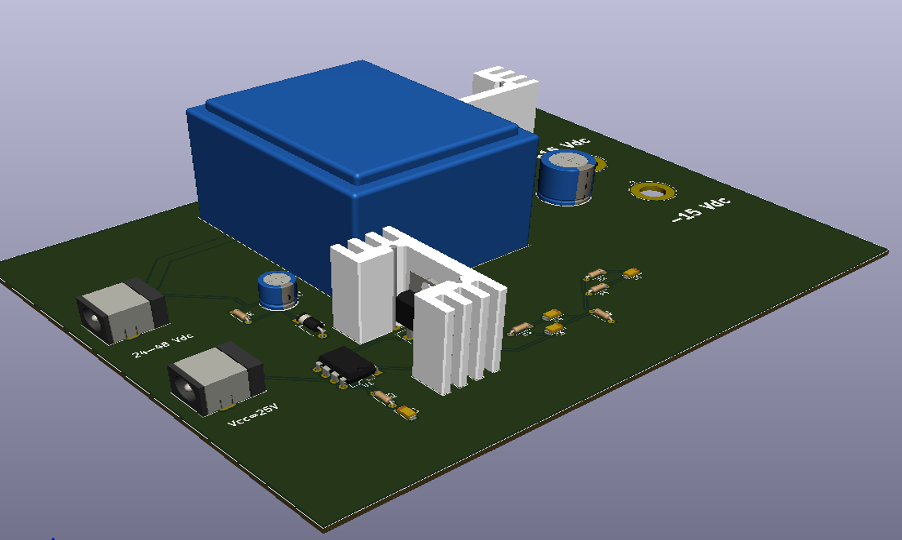
\includegraphics[scale=0.8]{PCB11.png}
    \caption{Side view of the circuit. }
    \label{fig:my_label}
\end{figure}








\section{Test Results }




\subsection{Line Regulation}


\subsubsection{With Controller}

\begin{figure}[H]
    \centering
    \includegraphics[scale=0.35]{24 to 48 v input(controlculu)(devre sematiği).png}
    \caption{Circuit schematic of LtSpice model with controller.}
    \label{fig:my_label}
\end{figure}


\begin{figure}[H]
    \centering
    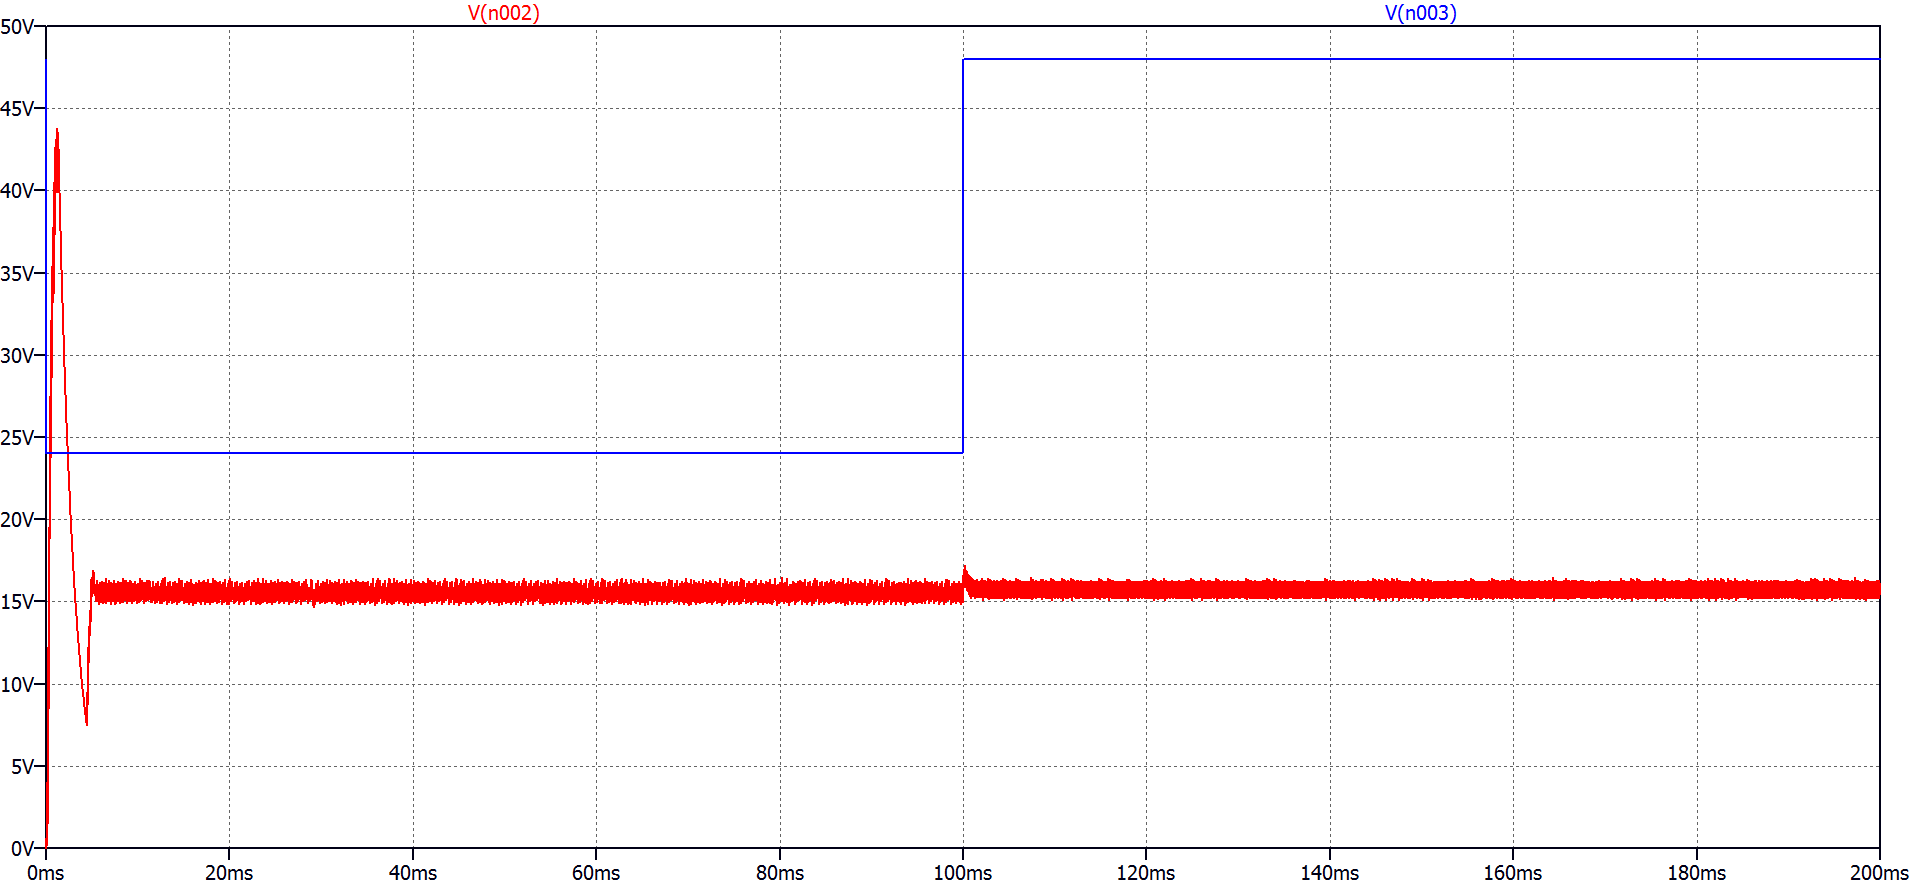
\includegraphics[scale=0.4]{24 to 48 v input(controlculu)(output voltage step response).png}
    \caption{Output step response with controller.}
    \label{fig:my_label}
\end{figure}

\begin{figure}[H]
    \centering
    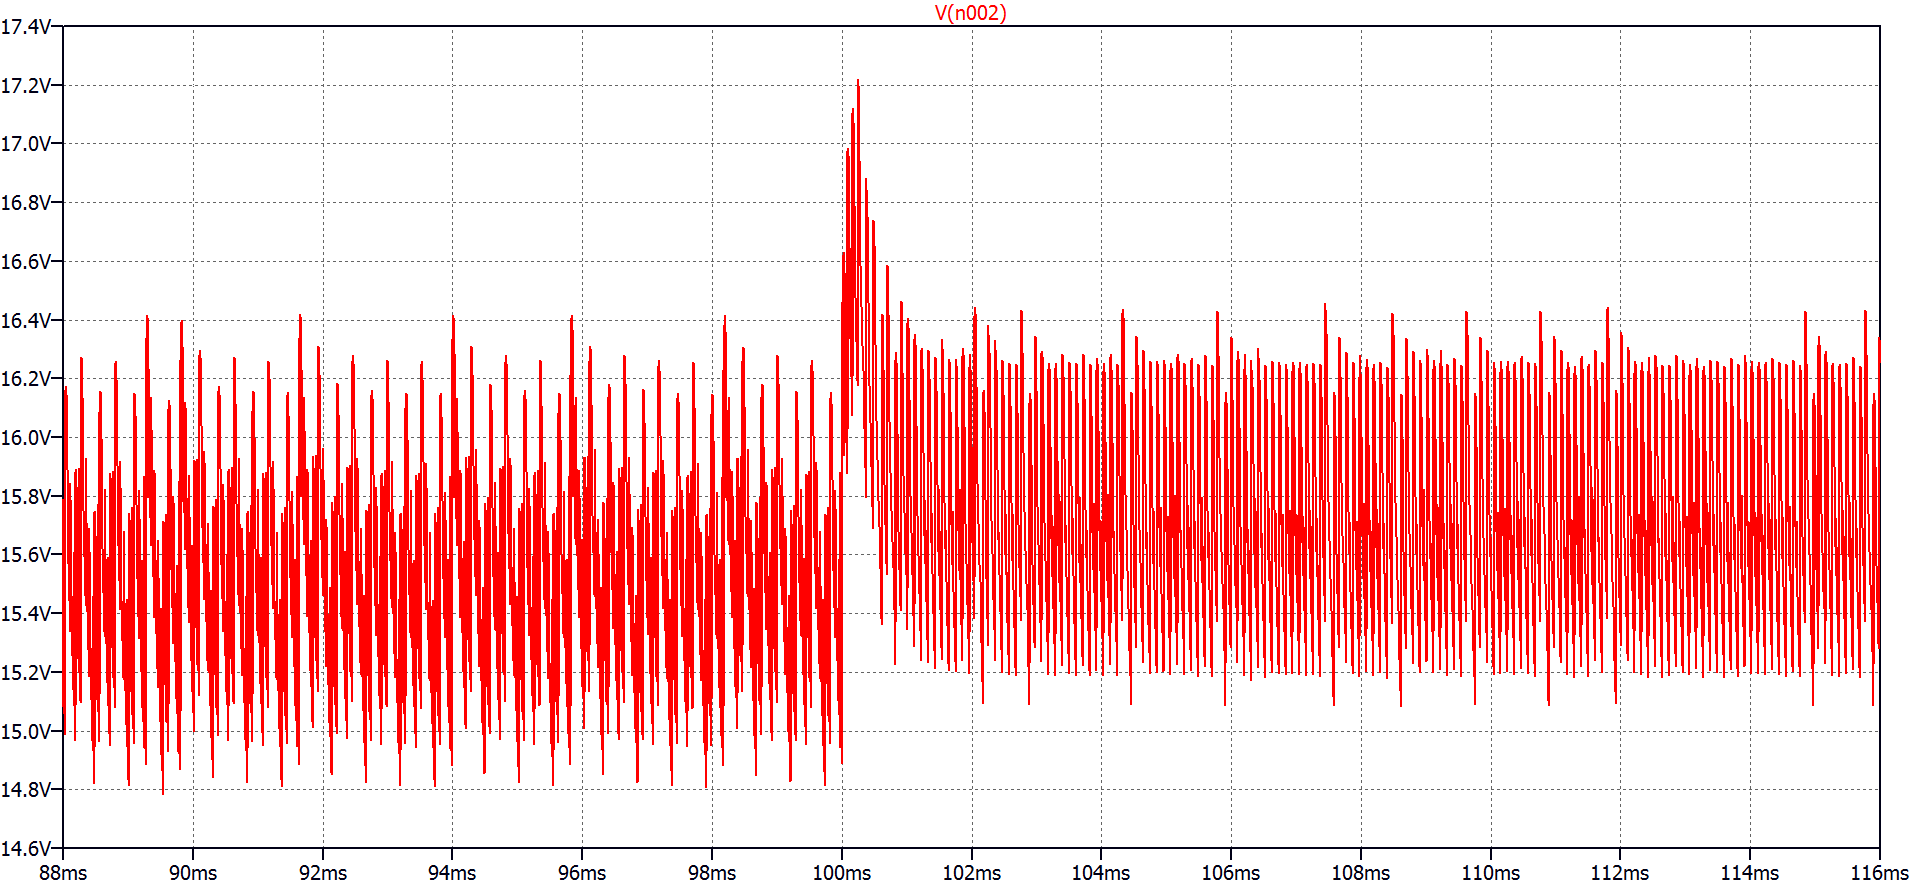
\includegraphics[scale=0.4]{24 to 48 v input(controlculu)(output voltage line regulation belli).png}
    \caption{More detailed output step response with controller.}
    \label{fig:my_label}
\end{figure}

\begin{figure}[H]
    \centering
    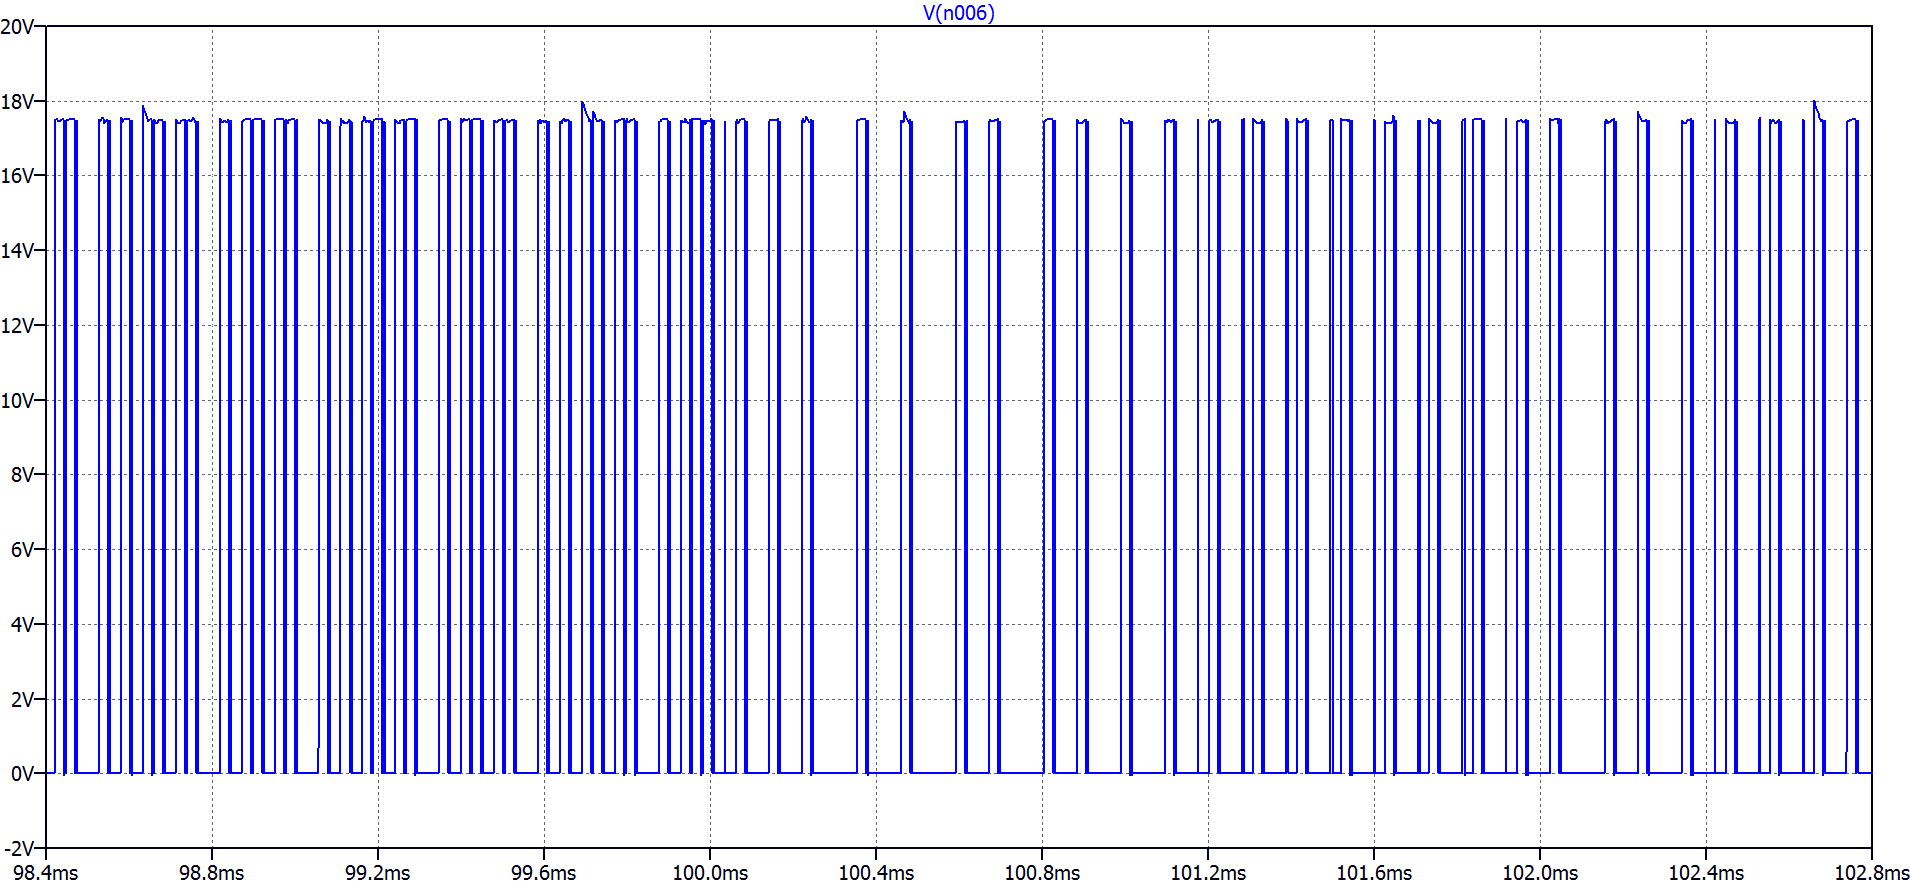
\includegraphics[scale=0.4]{24 to 48 v input(controlculu)(duty cycle).png}
    \caption{Duty cycle(gate signal) with controller.}
    \label{fig:my_label}
\end{figure}




\subsubsection{Without Controller}


\begin{figure}[H]
    \centering
    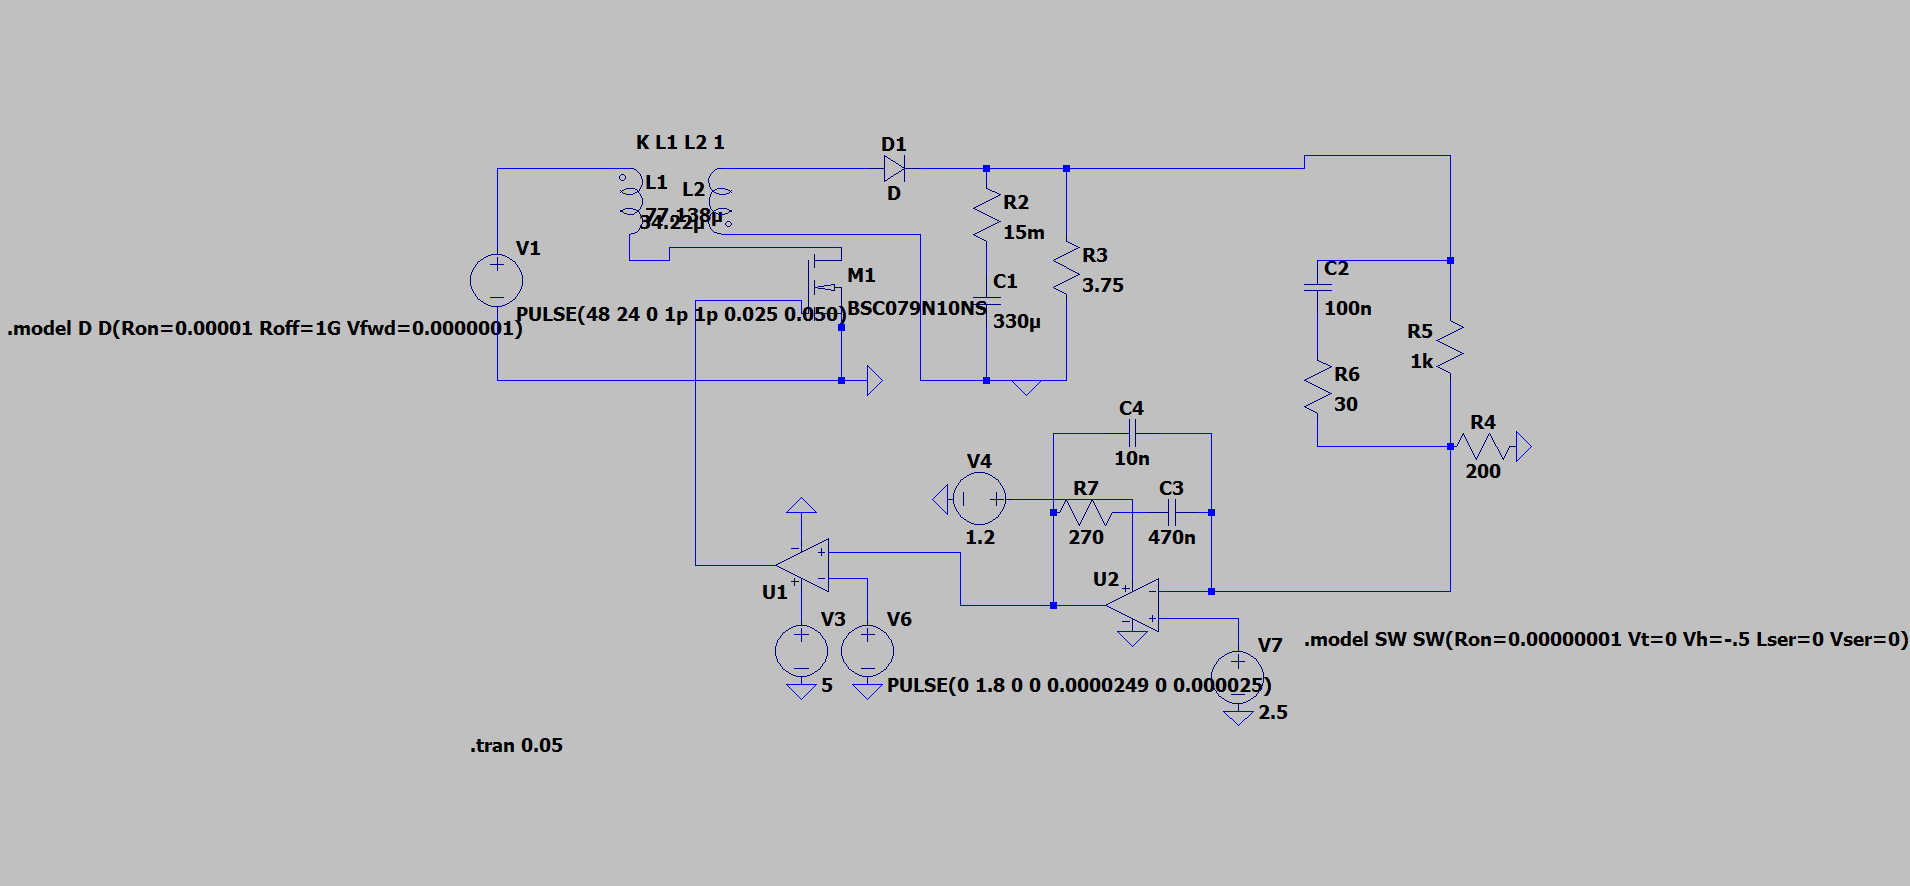
\includegraphics[scale=0.4]{24 to 48 v input(controlcu kullanmadan)(devre şematiğii.png}
    \caption{Circuit schematic of LtSpice model without controller.}
    \label{fig:my_label}
\end{figure}


\begin{figure}[H]
    \centering
    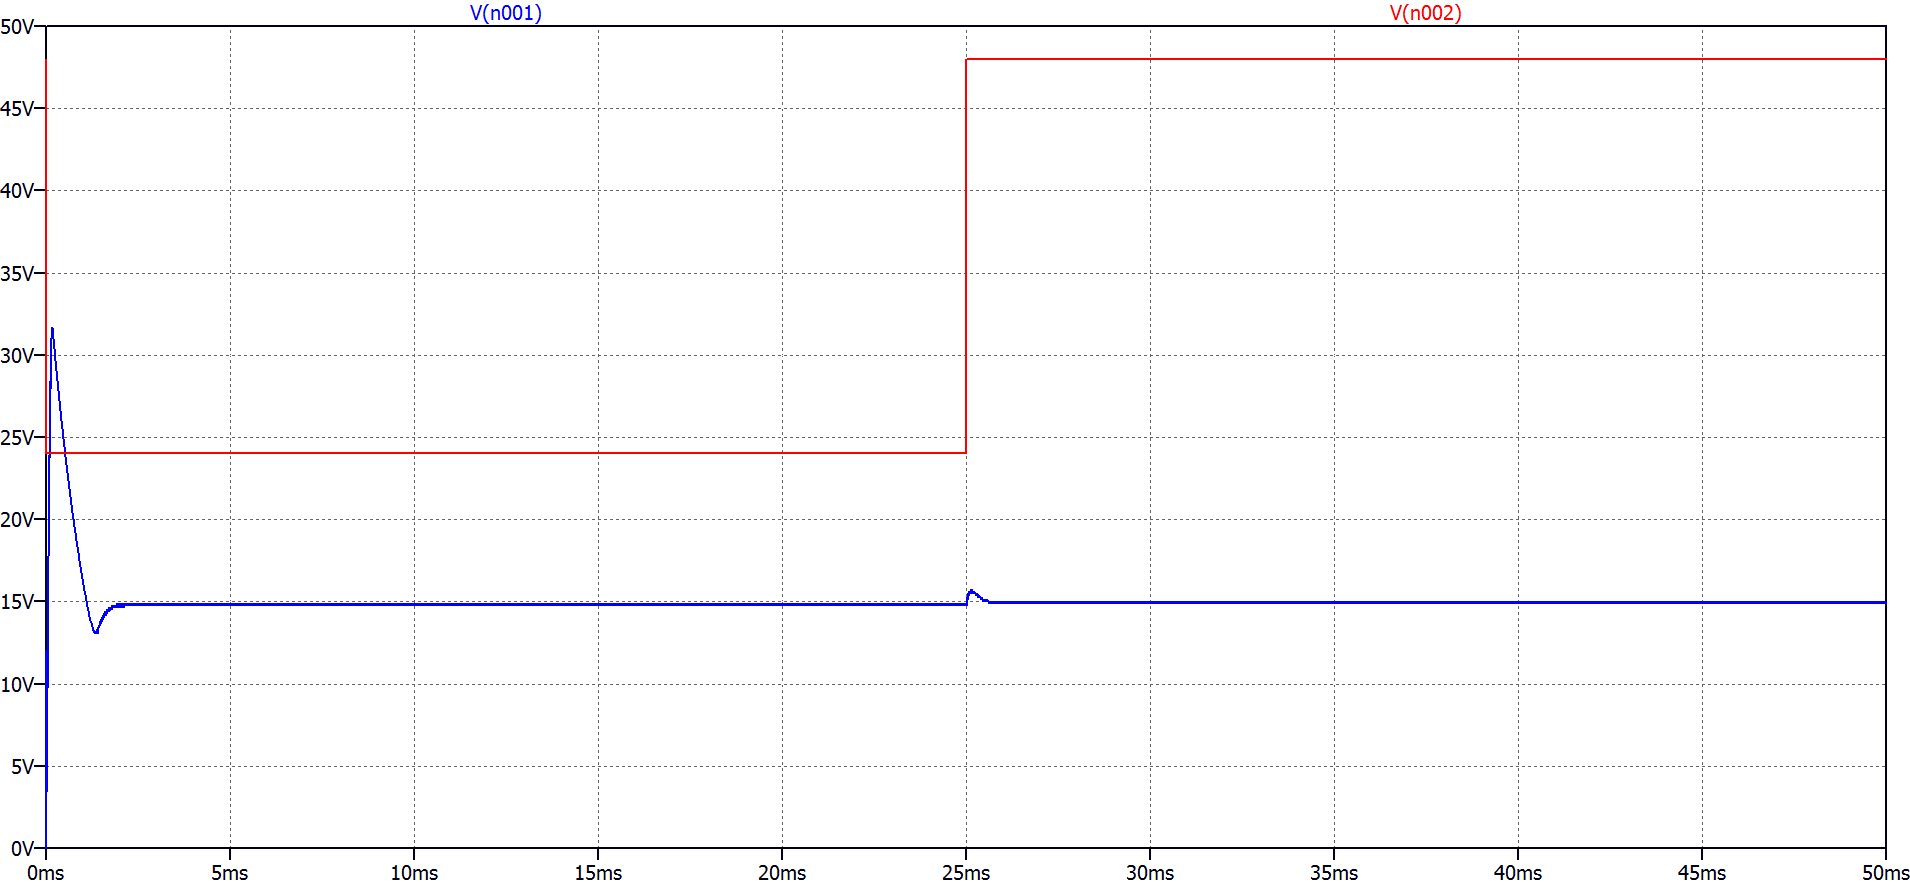
\includegraphics[scale=0.4]{24 to 48 v input(controlcu kullanmadan).PNG}
    \caption{Output step response without controller.}
    \label{fig:my_label}
\end{figure}

\begin{figure}[H]
    \centering
    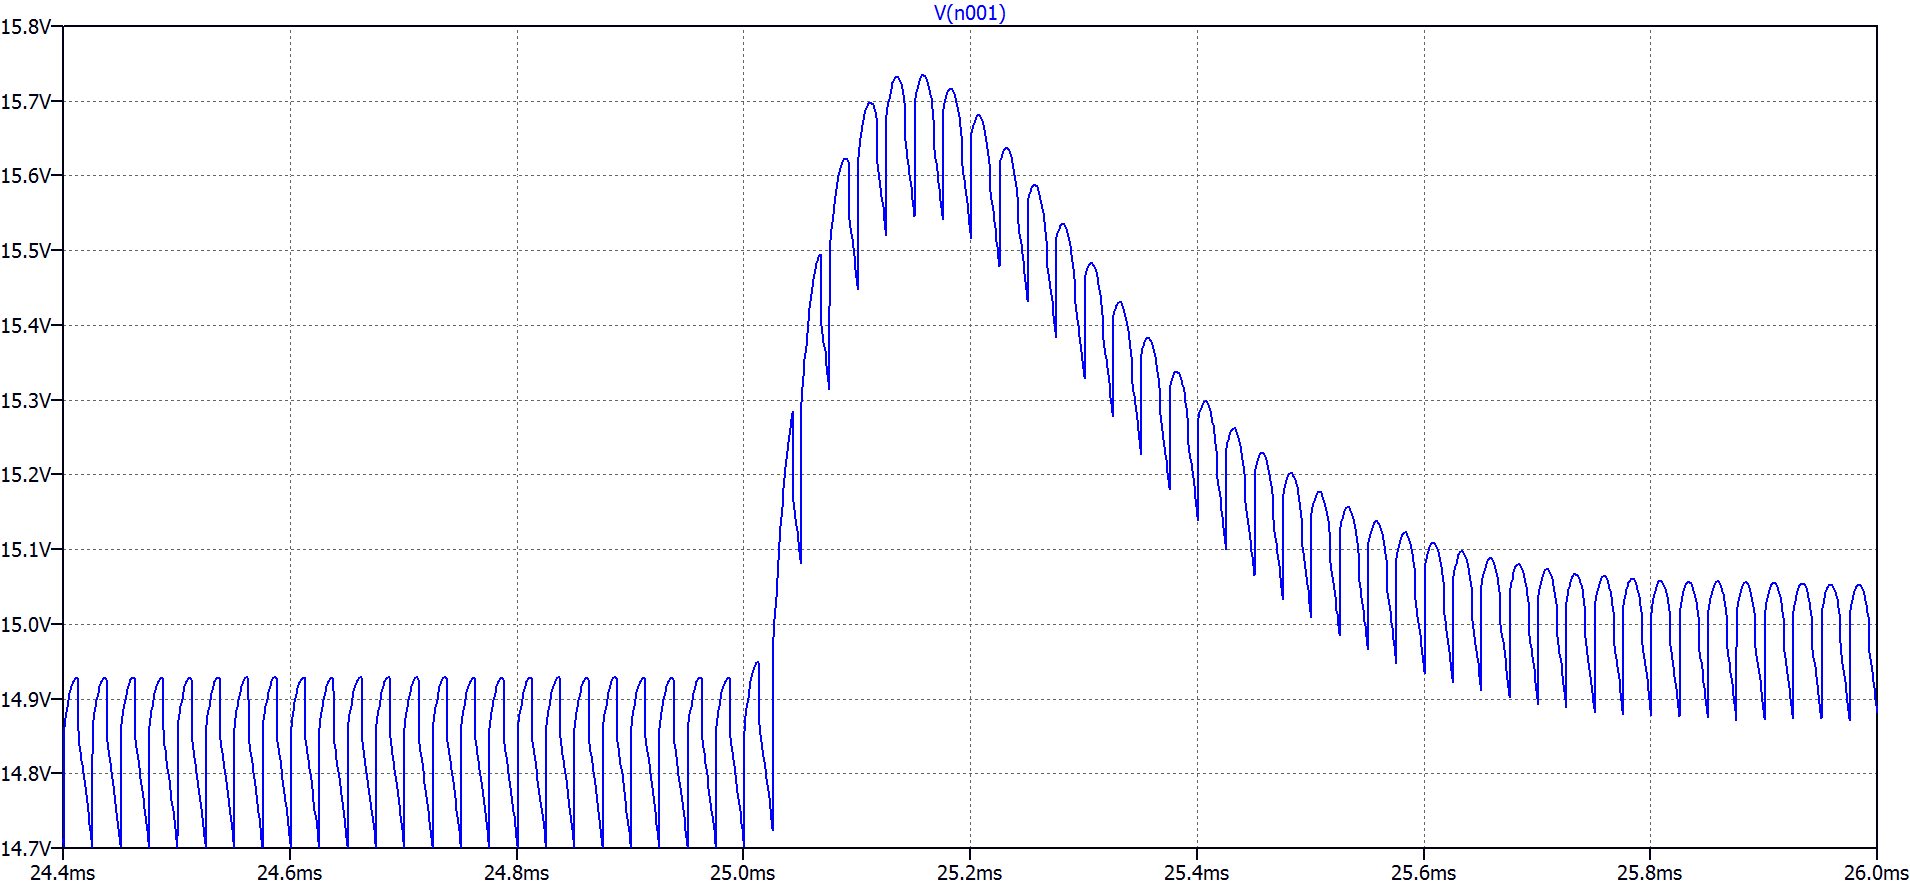
\includegraphics[scale=0.4]{24 to 48 v input(controlcu kullanmadan)-line regulation belli.png}
    \caption{More detailed output step response without controller.}
    \label{fig:my_label}
\end{figure}

\begin{figure}[H]
    \centering
    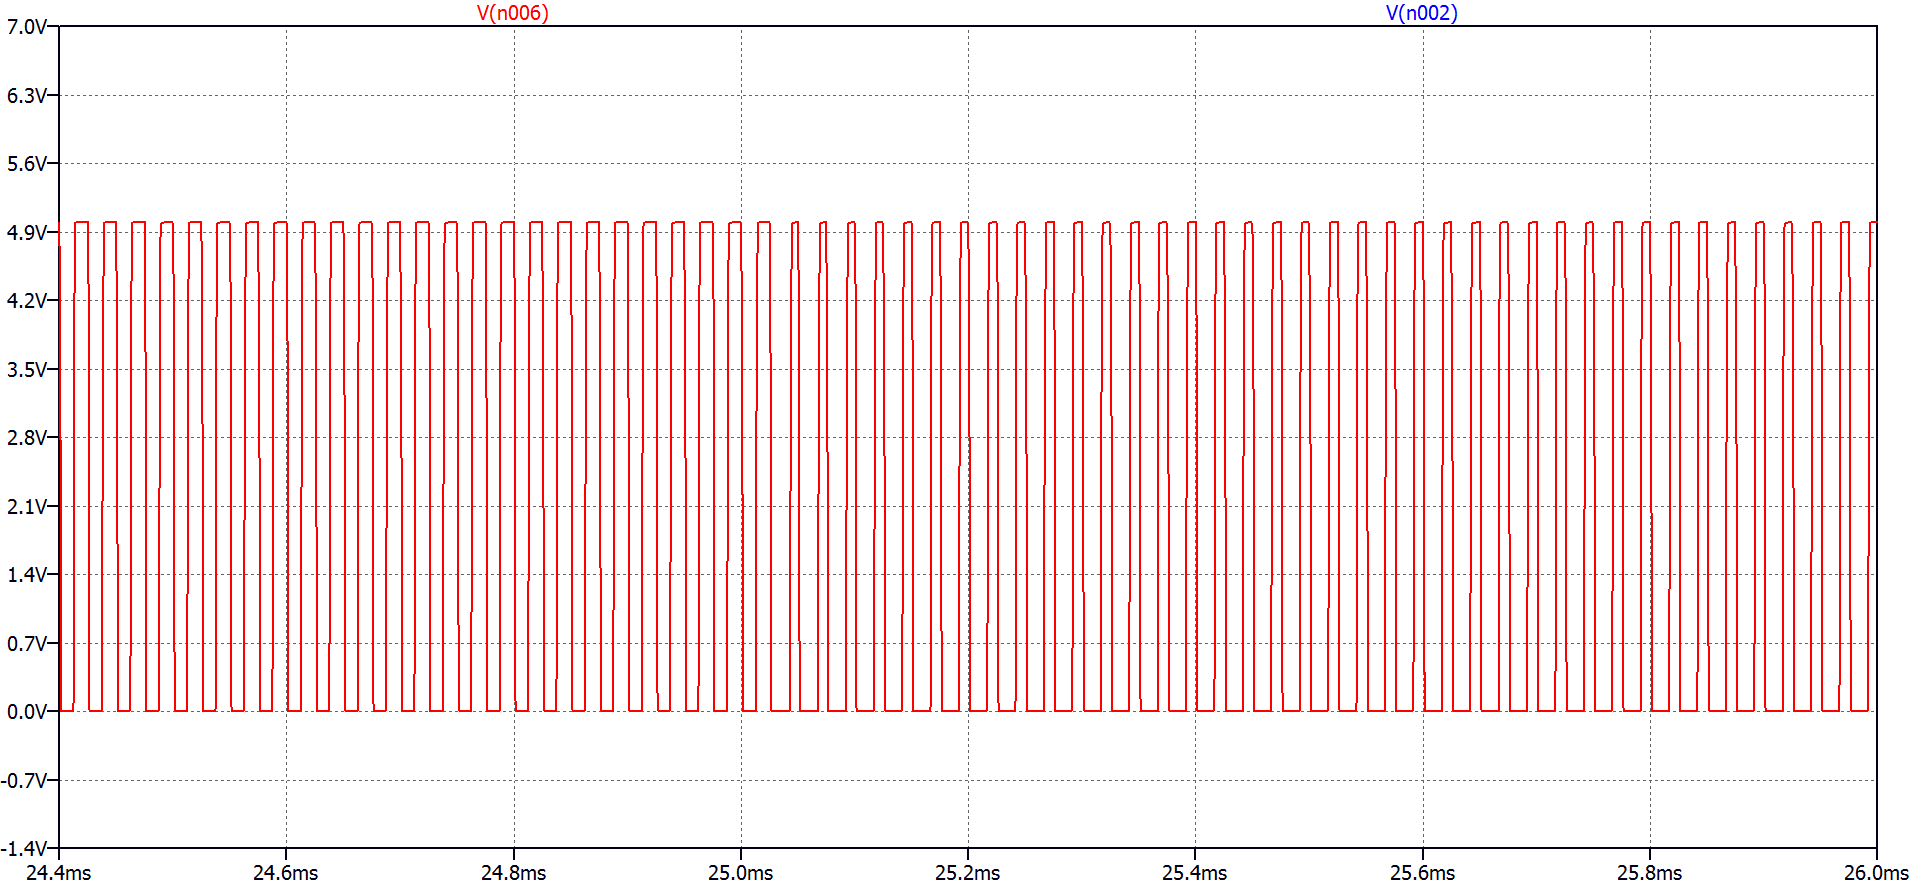
\includegraphics[scale=0.4]{24 to 48 v input(controlcu kullanmadan)(duty cycle.png}
    \caption{Duty cycle(gate signal) without controller.}
    \label{fig:my_label}
\end{figure}

\begin{figure}[H]
    \centering
    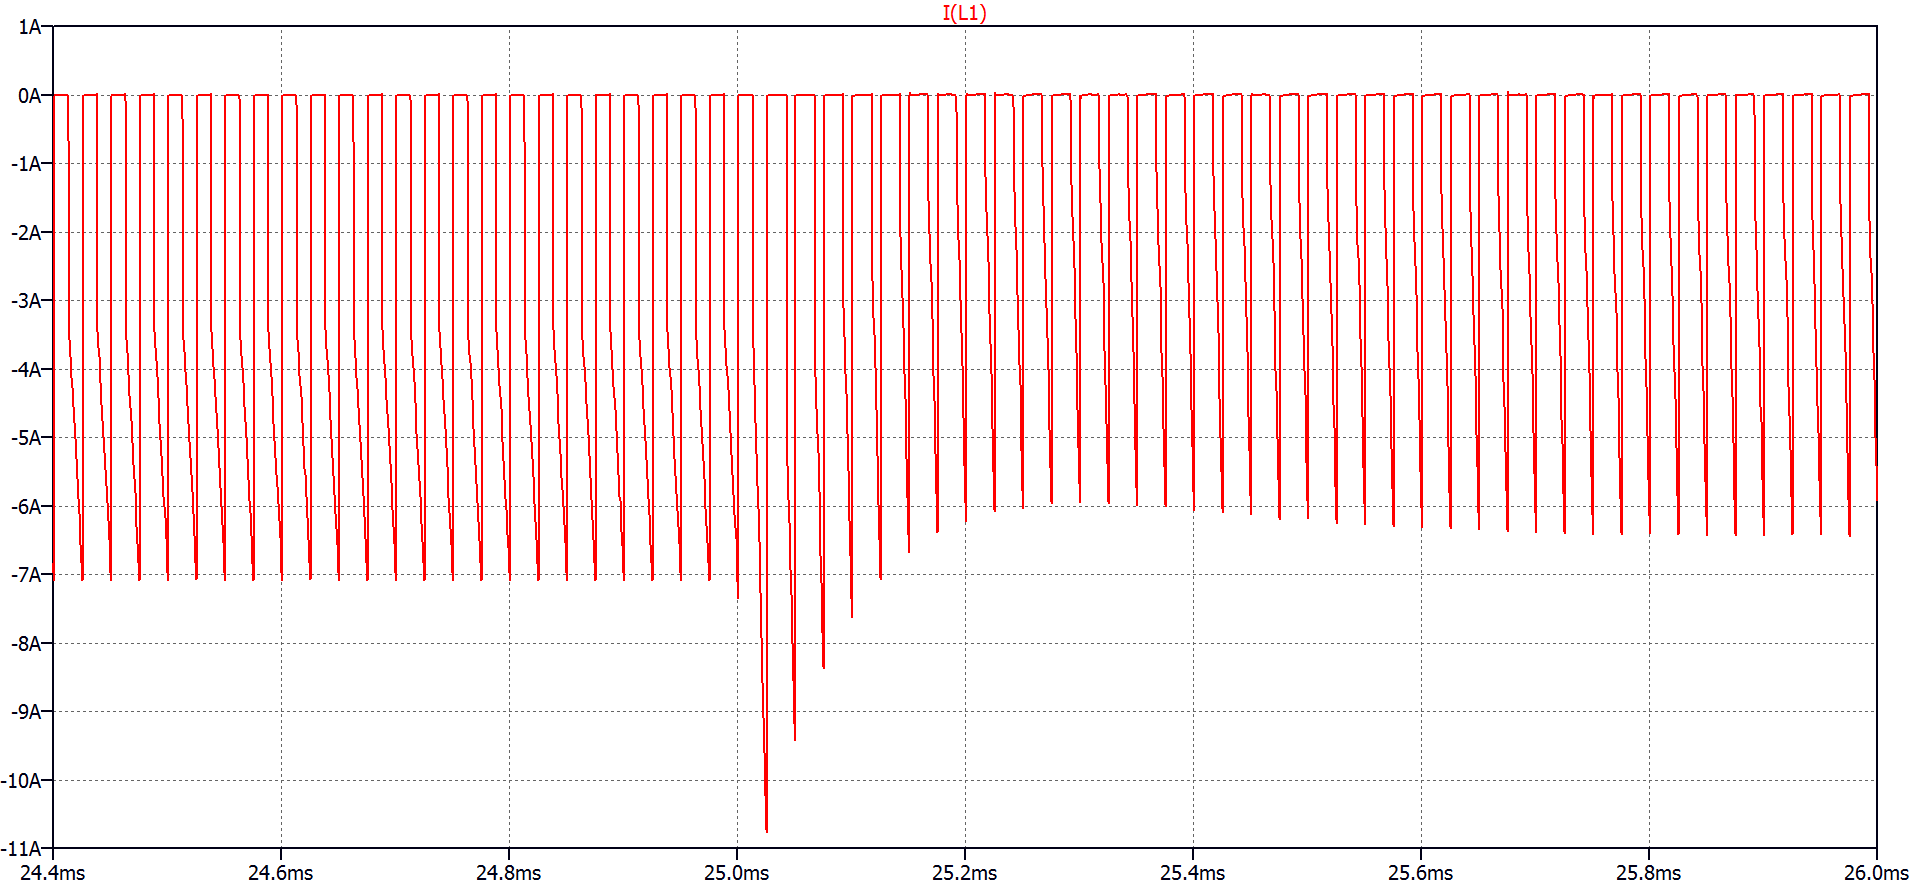
\includegraphics[scale=0.4]{24 to 48 v input(controlcu kullanmadan)(primary inductance current).png}
    \caption{Primary inductance current without controller.}
    \label{fig:my_label}
\end{figure}


\begin{figure}[H]
    \centering
    \includegraphics[scale=0.4]{24 to 48 v input(controlcu kullanmadan)(error amplifier output voltage.png}
    \caption{Error amplifier output without controller.}
    \label{fig:my_label}
\end{figure}

\subsection{Load Regulation Test}
  In order to test the load regulation of the system we simply connect a parallel load with the same resistance to the output. Initially, circuit starts with full-load or half-load but since there is a switch which series with the additional load, we can control its existence in the circuit. in other words we can make “On” and “OFF” to the mosfet thus connecting and disconnecting the parallel resistance at the output.
\subsubsection{Half load to full load}

\begin{figure}[H]
    \centering
    \includegraphics[scale=0.7]{e1.png}
    \caption{Half load to full load.}
    \label{fig:my_label}
\end{figure}


\subsubsection{Full load to half load}


\begin{figure}[H]
    \centering
    \includegraphics[scale=0.7]{e2.png}
    \caption{Full load to half load.}
    \label{fig:my_label}
\end{figure}


As we can see from the Figure 43 and 44, controller can react fastly and return the output voltage to its reference however returning may not be perfect since those controller are not perfect and are not linear in all the regions that the output value fallow.



\begin{figure}[H]
    \centering
    \includegraphics[scale=0.7]{e3.png}
    \caption{Measurement of the load regulation.}
    \label{fig:my_label}
\end{figure}
As can be seen from the Figure 43 and 44, difference between loads is 0.2 volt so,
$\frac{0.2}{15}=\%1.33$ load regulation  which is under \%2.




\subsection{Open-loop Transfer Function Verification Test}
In this test, the aim is verifying the analytically calculated transfer function by using a reliable software tool. For that purpose, we simply created a “Average Switch model” of the CCM flyback converter in the Matlab.
\begin{figure}[H]
    \centering
    \includegraphics{s1.png}
    \caption{Average switch model of flyback converter.}
    \label{fig:my_label}
\end{figure}


	By using that circuit, we just linearize the switch network which includes diode and mosfet however, there are still non-idealities in the circuit because we don’t exclude input voltage in that circuit. However, linearizing those nonlinearities would become much easier compared to original circuit because linearizing duty cycle is much more harder. 

	Therefore, as we can understand we simply use linearizing tool of the matlab to extract bode plot and transfer function of the open-loop system.
\begin{figure}[H]
    \centering
    \includegraphics[scale=0.8]{s2.png}
    \caption{Bode plot of average switch network when $V_{in}=36V$ .}
    \label{fig:my_label}
\end{figure}
\begin{figure}[H]
    \centering
    \includegraphics[scale=0.8]{s3.png}
    \caption{Extraction of transfer function from linearization tool.}
    \label{fig:my_label}
\end{figure}



As can be seen from the Figure 47 and 48, open-loop transfer functions are closely match with the analytical results.

\subsection{Mosfet Temperature Test}

  In this test, we have tried to find the correct value of the mosfets junction and case temperature and comparing it with the analytical results, for that purpose, 24 volt input is given (to create worst case condition) and in lt spice there is a heat sink model which we can create the one that we choose in simulation environment. whole circuit is like below.

\begin{figure}[H]
    \centering
    \includegraphics[scale=0.8]{t1.png}
    \caption{Thermal design simulation.}
    \label{fig:my_label}
\end{figure}


For that purpose, The junction to case and case junction resistances of the mosfer will be found which is similar to our mosfet, also, the found heatsink temperature resistance is also given.

\begin{figure}[H]
    \centering
    \includegraphics[scale=0.8]{t2.png}
    \caption{Tc junction.}
    \label{fig:my_label}
\end{figure}



From the above node(Tj) , we have measured the combined temperature of the junction
and results are as below.

\begin{figure}[H]
    \centering
    \includegraphics[scale=0.8]{t3.png}
    \caption{Junction temperature of the Mosfet.}
    \label{fig:my_label}
\end{figure}


\subsection{Snubber Test}

The test of the snubber circuit is made under the very detailed model of the Mosfet(IRF540N) to realize the real switching behaviour of the circuit together with the snubber circuit. Therefore, pre-calculated rise and fall time of the mosfet is realized by connected $C_{ds}$ capacitor. Moreover, since we have variable input range the test is done under the worst case condition for the highest voltage stress of the mosfet that can happen $Vin=48$.

\begin{figure}[H]
    \centering
    \includegraphics[scale=0.6]{wosnb.png}
    \caption{The voltage on switch without the snubber.}
    \label{fig:my_label}
\end{figure}

\begin{figure}[H]
    \centering
    \includegraphics[scale=0.6]{wsnb.png}
    \caption{The voltage on switch with the snubber.}
    \label{fig:my_label}
\end{figure}
\newpage
As can be seen from Figure 52 and 53, increase in the mosfet $V_{ds}$ voltage is confined in small value thanks to voltage keeping behaviour of the snubber capacitor.\\

 We have 100V rated mosfet(IRF540N) so it is clear that chosen component can withstand these conditions.\\



\section{Bill of Materials}

\begin{figure}[H]
    \centering
    \includegraphics[scale=0.4]{BOM.png}
    \caption{All components list.}
    \label{fig:my_label}
\end{figure}


\subsection{Component Selection}

\subsubsection{Power Handling Components}

Mosfet:\\
As mentioned before, since rectifier operates in CCM. In order to reduce the conduction losses, a MOSFET having small ON resistance is selected.
Maximum current flowing through the MOSFET is primary side peak current. Although considering RMS current is pretty enough during component selection, peak currents provides some margin and more reliable operation. Therefore,\\
$I_{rated(Mosfet)} > I_{pri(peak)} = 6.6A$

 Voltage rating of the MOSFET is calculated as follows: \\
$V_{rated(Mosfet)} = V_{in,max} + V_R + V_{spike}$\\
Assuming expected maximum spike voltage is 30 \% of maximum input voltage. Note that that spikes are decreased with a clamp circuit.\\
$V_{rated(Mosfet)} =48 + 31 + 14.4 = 93.4V$\\
For that purpose, 100V 33A 0.044 ohm “IRF540NSPbF” .\\
Output Diode:\\
Similarly, in order to decrease the conduction losses, a schottky diode is chosen. and since it is fast recovery time its switching losses are also low.

$V_{rated(diode)} = V_{out}+ V_{in,max}N_{sec} N_{pri}= 39V$

$I_{rated(diode)}> I_{sec(peak)} = 11.32A$

Secondary peak current is considered due to more reliable operation.\\ Moreover, 30\% margin is added to voltage rating. At the end, a schottky diode whose ratings are over 50V and 22.32 A is selected. For this purpose, 80 V 30 A VT3080S is chosen. It’s forward voltage drop is typically 0.5-0.6 V.

\subsubsection{Snubber Components}

Resistor: \\Most critical component of the snubber is the resistor because it should dissipate the power which is coming from the leakage inductance. and in the snubber part finding required resistor is derived so, it is 2k ohm. and it since the voltage on the capacitor is around 20-22.5 V, it passes around 10 mA current continuously, so it dissipates about 0.2 watt power. in order to realize that operation, we choose “ PPC1.0KW-2TR-ND” 1 kohm but 2 in series, each one of them has power rating of 2W, so it can handle that operation.


Capacitor: \\Capacitor value of the snubber is not that critical beacause as long as it can keep the voltage of itself during the switching period it means no matter the value, it can be useful in snubber circuit. Also, since it will be parallel to the primary winding during the “OFF” time of the mosfet it can bear the “Flyback” voltage so, for our circuit, its voltage rating should be around 20-25V for that purpose, we have chosen the “TVA207.7” $ 200\mu F $which has 25 Volt rating.

Diode: \\Diode ratings are not that important for the current values because if we assume that there is zero average current passing through the capacitor average current passign through diode will be 10 mA but when it is off it can withstand $V_{in}-V_{cap}(V_{flyback})=$ around 1.5 volt to 25.5 Volt to work properly, So,we choose, “1N4007” diode which has “1000 Vrrm” and “1 amp” average current rating.




\subsubsection{Filter Components}


Capacitor: Since rectifier is operating on DCM, and higher peak currents flow through the components, ESR of the capacitor becomes important.
$C_{cap} >>I_{out}D_{max} f_{sw}V_{ripple}$.\\
$N_{cp}$ is a value between 10-20, and allowable maximum ripple for that case is 0.6 V. Taking it as 10,\\
$C_{min} = 9.3\mu F$\\
Calculating maximum ESR:\\
$ESR_{max} =V_{ripple} I_{sec(peak)}= 0.0268\Omega$

$V_{rated(cap)} = V_{out} = 15V$
At the end, 50 V 330 $\mu F $ $ 23 m\Omega$ aluminium electrolytic capacitor is chosen.



\subsubsection{Integrated Circuits}
PWM Controller:\\
In order to make regulation for the output voltage, we need a some kind of feedback to some reference value, For that purpose, instead of using opamps to realize error amplifier, we have used “LT1246” PWM modulator. It has a wide range of oscillator frequency including the one that we have choose for the implementation which is 40kHz.
\begin{figure}[H]
    \centering
    \includegraphics{IC.png}
    \caption{Error amplifier of the Lt1246.}
    \label{fig:my_label}
\end{figure}

It has its own internal error amplifier, which has a reference voltage of 2.5 Volt, therefore, in order to regulate 15 volt output voltage, we need to divide that value to be equal to 2.5 volt by creating voltage divider network. Also it has a “RT/CT” pin that can be connected to an “RC” circuit to adjusting its ramp waveform frequency.

\subsubsection{Compensator Network}

First of all, all of the component that are connected to this network is end up at the pins which are “FB” and “COMP” both of are input to the some operational amplifiers inside the controller therefore the current passing through these components is not among the selection considerations. However, during the start-up, the voltage on the output can reach the 45 volt therefore, their rating may be at least that value to guarantee the safe operation because we don’t have any isolation on the feedback side.\\

Voltage divider network:\\ This part is also included in compensation network it consists of two resistors which are 1k and 200 ohm. as we mention above, their current rating are not important. So, we choose “CF14JT200R” as 200 ohm and “PR02000201001JR500” as 1kohm.\\

Compensation network: \\The components that are related to that part is derived in the “compensator” section. So in here we are just sharing the products as round values of previously calculated numbers. However, since there is no power handling and regulating high voltages (i.e output capacitor of circuit) all the capacitors are chosen as “Ceramic” capacitors.\\470nF capacitor :C0402C474K9PACTU\\
10nF capacitor   :GRM155R71C103KA01J\\
100nF capacitor  :C0402C102K5RACTU\\
270 $\Omega$ resistor  :CF14JT270R\\
30 $\Omega$resistor :  CFR-25JB-52-30R\\

\subsubsection{Oscillator}

In the Oscillator part , choosing the component values as close as the founded values in the paper is really important because it determines our switching frequency. we have made this calculation using the given equations in the controller datasheet as below:
\begin{gather*}
    \text{Oscillator rise time:} t_r=0.583RC\\
    \text{Oscillator discharge time:} t_d=\frac{3.46RC}{0.0164R-11.73}\\
    \text{Oscillator period:}t_{osc}=t_r+t_d\\
\end{gather*}

So, in our case $T_{osc}=25 \mu sec$ therefore equating this number to above formulas gives that :\\
\begin{gather*}
   R=1k\Omega\\
C=18.8 nF \text{(choose it as 18nF) }
\end{gather*}


So the chosen components are as below:\\

R = (PR02000201001JR500)\\
C = (C0603C183K5RACTU) 

\section{Conclusion}

In that project, a Flyback converter with certain specifications is designed. Before starting to the design process, a very comprehensive research has been done. All necessary points of the design is considered, and the best solution is tried to develop between countless trade-offs. Actually, these points are not just conceptual ideas but also the design arguments that are supported by very detailed simulation results. In simulation step, we have used many different software such as TINA, SIMPLIS, KicadAlso etc. Also, an excel sheet is formed to understand the trade-offs of the system better. Eventually, the design is successfully completed under the software tools which are mainly Simulink and LtSpice. This report gives an information about the what we have did during the semester for that project. It includes very detailed design information from circuit configurations to component selections and not only under the simulation environment but also  it includes explanation of the producible PCB design that is created by us. Moreover, in the design part, we explain how we achieve the requirements of that topology how we overcome the challenges of the design and how much effort we make during the design process  and in the test result part, we have showed that we did the job with all of the specifications and verify that this system is working as we have designed.

\section{References}

[1]= Kool Mµ® Material Curves. (n.d.). Retrieved from https://www.mag-inc.com/Products/Powder-Cores/Kool-Mu-Cores/Kool-Mu-Material-Curves
\newline
[2]= (n.d.). Retrieved from https://www.mag-inc.com/Media/Magnetics/Datasheets/00K3515E090.pdf 
\newline
[3]= (n.d.). Retrieved from https://www.mag-inc.com/Media/Magnetics/File-Library/Product%20Literature/Powder%20Core%20Literature/Magnetics-Kool-Mu-MAX-Bulletin.pdf
\newline
[4]= (n.d.). Retrieved from https://pdf.direnc.net/upload/irf540nspbf-datasheet.pdf
\newline
[5]= (n.d.). Retrieved from http://www.vishay.com/docs/89242/vt3080s.pdf
\newline
[6]= (n.d.). Retrieved from https://www.mouser.com.tr/datasheet/2/315/ABA0000C1255-1128316.pdf
\newline
[7]=(n.d.). Retrieved from https://www.monolithicpower.com/en/documentview/productdocument/index/version/2/document_type/Application%20Note/lang/en/sku/MP020-5/document_id/2307

\end{document}